   \documentclass{article}
\usepackage{pgfplots}
\begin{document}
\begin{figure}
\centering

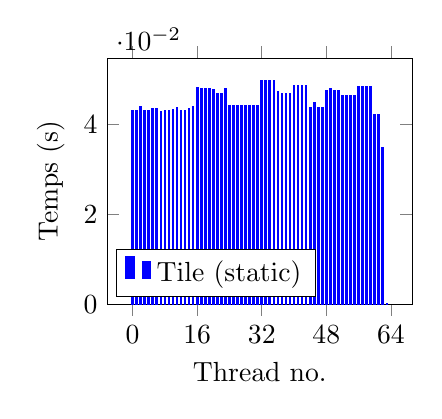
\begin{tikzpicture}
\begin{axis}[
  ybar,
  bar width=0.02cm,
  xlabel={Thread no.},
  ylabel={Temps (s)},
  ymin=0,
  legend pos=south west,
  width=0.45\textwidth,
  xtick distance=16
]

% Données pour le premier graphique (à gauche)
\addplot[color=blue, fill=blue] coordinates {
  (0,0.043148) (1,0.043153) (2,0.044079) (3,0.043156) (4,0.043034) (5,0.043528) (6,0.043516) (7,0.043005) (8,0.043222) (9,0.043241) (10,0.043379) (11,0.043781) (12,0.043211) (13,0.043211) (14,0.043633) (15,0.043943) (16,0.048203) (17,0.048008) (18,0.048032) (19,0.048045) (20,0.047767) (21,0.046974) (22,0.046982) (23,0.048050) (24,0.044262) (25,0.044300) (26,0.044283) (27,0.044239) (28,0.044271) (29,0.044276) (30,0.044258) (31,0.044300) (32,0.049815) (33,0.049840) (34,0.049811) (35,0.049813) (36,0.047295) (37,0.046925) (38,0.047003) (39,0.046939) (40,0.048644) (41,0.048631) (42,0.048630) (43,0.048631) (44,0.043753) (45,0.044959) (46,0.043752) (47,0.043802) (48,0.047672) (49,0.047999) (50,0.047679) (51,0.047653) (52,0.046525) (53,0.046536) (54,0.046525) (55,0.046519) (56,0.048493) (57,0.048501) (58,0.048492) (59,0.048522) (60,0.042178) (61,0.042197) (62,0.034897) (63,0.000055)
};
\addlegendentry{Tile (static)}

\end{axis}
\end{tikzpicture}
\hfill
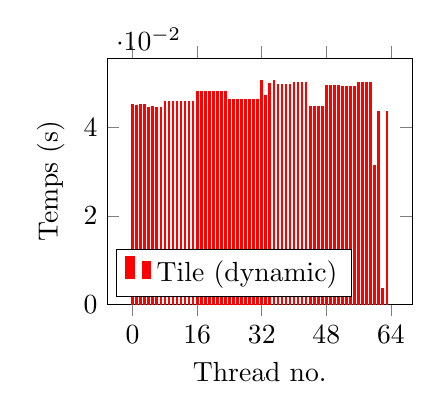
\begin{tikzpicture}
\begin{axis}[
  ybar,
  bar width=0.02cm,
  xlabel={Thread no.},
  ylabel={Temps (s)},
  ymin=0,
  legend pos=south west,
  width=0.45\textwidth,
  xtick distance=16
]

% Données pour le deuxième graphique (au milieu)
\addplot[color=red, fill=red] coordinates {
  (0,0.045119) (1,0.045073) (2,0.045118) (3,0.045115) (4,0.044508) (5,0.044726) (6,0.044512) (7,0.044501) (8,0.045910) (9,0.045897) (10,0.045902) (11,0.045902) (12,0.045785) (13,0.045776) (14,0.045784) (15,0.045776) (16,0.048125) (17,0.048147) (18,0.048153) (19,0.048138) (20,0.048158) (21,0.048159) (22,0.048150) (23,0.048135) (24,0.046223) (25,0.046231) (26,0.046228) (27,0.046232) (28,0.046230) (29,0.046230) (30,0.046219) (31,0.046219) (32,0.050641) (33,0.047188) (34,0.049958) (35,0.050626) (36,0.049655) (37,0.049655) (38,0.049674) (39,0.049657) (40,0.050069) (41,0.050072) (42,0.050074) (43,0.050068) (44,0.044747) (45,0.044734) (46,0.044734) (47,0.044732) (48,0.049437) (49,0.049430) (50,0.049427) (51,0.049425) (52,0.049372) (53,0.049352) (54,0.049363) (55,0.049364) (56,0.050263) (57,0.050263) (58,0.050274) (59,0.050264) (60,0.031317) (61,0.043666) (62,0.003443) (63,0.043672)
};
\addlegendentry{Tile (dynamic)}

\end{axis}
\end{tikzpicture}
\hfill
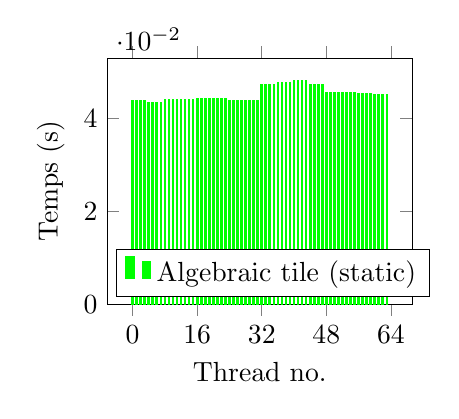
\begin{tikzpicture}
\begin{axis}[
  ybar,
  bar width=0.02cm,
  xlabel={Thread no.},
  ylabel={Temps (s)},
  ymin=0,
  legend pos=south west,
  width=0.45\textwidth,
  xtick distance=16
]

% Données pour le troisième graphique (à droite)
\addplot[color=green, fill=green] coordinates {
  (0,0.043828) (1,0.043848) (2,0.043844) (3,0.043845) (4,0.043520) (5,0.043500) (6,0.043518) (7,0.043512) (8,0.044049) (9,0.044042) (10,0.044043) (11,0.044047) (12,0.044046) (13,0.044033) (14,0.044029) (15,0.044040) (16,0.044382) (17,0.044357) (18,0.044381) (19,0.044399) (20,0.044388) (21,0.044374) (22,0.044370) (23,0.044388) (24,0.043854) (25,0.043824) (26,0.043852) (27,0.043865) (28,0.043859) (29,0.043831) (30,0.043856) (31,0.043866) (32,0.047350) (33,0.047335) (34,0.047344) (35,0.047356) (36,0.047855) (37,0.047838) (38,0.047852) (39,0.047850) (40,0.048203) (41,0.048188) (42,0.048206) (43,0.048216) (44,0.047415) (45,0.047413) (46,0.047411) (47,0.047412) (48,0.045655) (49,0.045627) (50,0.045642) (51,0.045645) (52,0.045665) (53,0.045639) (54,0.045685) (55,0.045664) (56,0.045358) (57,0.045321) (58,0.045353) (59,0.045357) (60,0.045279) (61,0.045229) (62,0.045263) (63,0.045279)
};
\addlegendentry{Algebraic tile (static)}

\end{axis}
\end{tikzpicture}

\caption{Temps d'exécution des threads pour le fichier gemm.c}
\label{fig:graphes}
\end{figure}

\begin{table}[htbp]
  \centering
  \caption{Statistiques pour le fichier gemm.c}
  \begin{tabular}{|c|c|c|c|}
    \hline
    Statistique & Algebraic Tile & Tile (static) & Tile (dynamic) \\ 
    \hline
    Skewness (g1)  & 0.676046 & -5.79426 & -5.52637 \\ 
    Kurtosis (g2)  & -1.00053 & 38.773 & 35.0313 \\ 
    Coefficient de variation $ \frac{\sigma}{\overline{x}} $ & 0.0341242 & 0.139027 & 0.132364\\ 
    Percent Imbalance metric en \% & 6.46294 & 10.7873 & 8.94216\\ 
    Coefficient de Gini  & 0.0186636 & 0.0466535 & 0.0443046\\ 
    Temps d'exécution (s) &  0.048278    &  0.049923   &  0.050854   \\ 

    \hline
  \end{tabular}
\end{table}
g1=$ \frac{\sum_{i=1}^{n} (x_i - \overline{x})^3}{n\sigma^3} $\
g2=$ \frac{\sum_{i=1}^{n} (x_i - \overline{x})^4}{n\sigma^4} $\
Coefficient de Gini = $ \frac{\sum_{i=1}^{n}\sum_{j=1}^{n} |x_i - x_j|}{2n^2\overline{x}} $\
\newpage

\begin{figure}
\centering

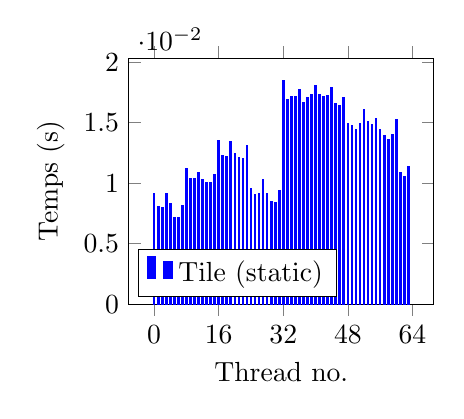
\begin{tikzpicture}
\begin{axis}[
  ybar,
  bar width=0.02cm,
  xlabel={Thread no.},
  ylabel={Temps (s)},
  ymin=0,
  legend pos=south west,
  width=0.45\textwidth,
  xtick distance=16
]

% Données pour le premier graphique (à gauche)
\addplot[color=blue, fill=blue] coordinates {
  (0,0.009141) (1,0.008031) (2,0.008000) (3,0.009180) (4,0.008288) (5,0.007174) (6,0.007163) (7,0.008175) (8,0.011205) (9,0.010407) (10,0.010368) (11,0.010919) (12,0.010320) (13,0.010020) (14,0.010058) (15,0.010745) (16,0.013522) (17,0.012282) (18,0.012201) (19,0.013473) (20,0.012495) (21,0.012144) (22,0.012062) (23,0.013081) (24,0.009555) (25,0.009101) (26,0.009139) (27,0.010267) (28,0.009145) (29,0.008468) (30,0.008414) (31,0.009428) (32,0.018496) (33,0.016957) (34,0.017200) (35,0.017187) (36,0.017709) (37,0.016711) (38,0.017124) (39,0.017326) (40,0.018052) (41,0.017351) (42,0.017158) (43,0.017247) (44,0.017937) (45,0.016580) (46,0.016465) (47,0.017071) (48,0.014966) (49,0.014758) (50,0.014440) (51,0.014921) (52,0.016085) (53,0.015098) (54,0.014823) (55,0.015374) (56,0.014444) (57,0.013911) (58,0.013579) (59,0.014063) (60,0.015290) (61,0.010856) (62,0.010513) (63,0.011415)
};
\addlegendentry{Tile (static)}

\end{axis}
\end{tikzpicture}
\hfill
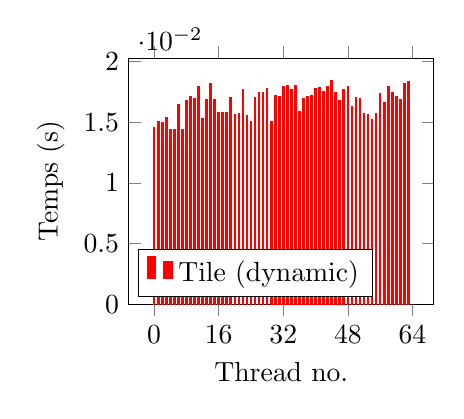
\begin{tikzpicture}
\begin{axis}[
  ybar,
  bar width=0.02cm,
  xlabel={Thread no.},
  ylabel={Temps (s)},
  ymin=0,
  legend pos=south west,
  width=0.45\textwidth,
  xtick distance=16
]

% Données pour le deuxième graphique (au milieu)
\addplot[color=red, fill=red] coordinates {
  (0,0.014585) (1,0.015089) (2,0.014944) (3,0.015361) (4,0.014406) (5,0.014433) (6,0.016499) (7,0.014446) (8,0.016817) (9,0.017108) (10,0.016983) (11,0.017960) (12,0.015288) (13,0.016881) (14,0.018169) (15,0.016882) (16,0.015843) (17,0.015801) (18,0.015844) (19,0.017031) (20,0.015638) (21,0.015728) (22,0.017708) (23,0.015603) (24,0.015072) (25,0.017025) (26,0.017426) (27,0.017473) (28,0.017821) (29,0.015105) (30,0.017184) (31,0.017101) (32,0.017980) (33,0.018008) (34,0.017737) (35,0.017997) (36,0.015888) (37,0.016967) (38,0.017125) (39,0.017175) (40,0.017808) (41,0.017912) (42,0.017561) (43,0.017995) (44,0.018454) (45,0.017479) (46,0.016833) (47,0.017696) (48,0.017949) (49,0.016307) (50,0.017024) (51,0.016978) (52,0.015692) (53,0.015678) (54,0.015244) (55,0.015705) (56,0.017397) (57,0.016640) (58,0.017923) (59,0.017473) (60,0.017131) (61,0.016885) (62,0.018192) (63,0.018395)
};
\addlegendentry{Tile (dynamic)}

\end{axis}
\end{tikzpicture}
\hfill
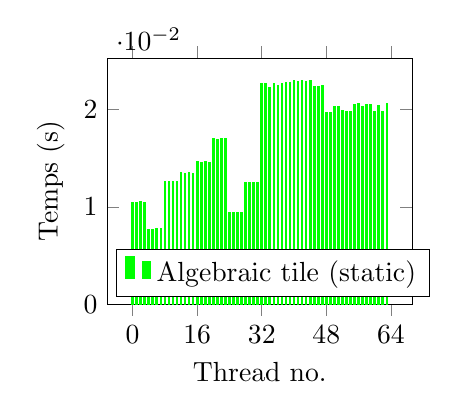
\begin{tikzpicture}
\begin{axis}[
  ybar,
  bar width=0.02cm,
  xlabel={Thread no.},
  ylabel={Temps (s)},
  ymin=0,
  legend pos=south west,
  width=0.45\textwidth,
  xtick distance=16
]

% Données pour le troisième graphique (à droite)
\addplot[color=green, fill=green] coordinates {
  (0,0.010504) (1,0.010493) (2,0.010551) (3,0.010485) (4,0.007685) (5,0.007665) (6,0.007788) (7,0.007756) (8,0.012603) (9,0.012562) (10,0.012624) (11,0.012570) (12,0.013489) (13,0.013433) (14,0.013501) (15,0.013438) (16,0.014632) (17,0.014595) (18,0.014632) (19,0.014593) (20,0.017037) (21,0.016973) (22,0.017081) (23,0.017000) (24,0.009470) (25,0.009411) (26,0.009449) (27,0.009406) (28,0.012540) (29,0.012483) (30,0.012527) (31,0.012476) (32,0.022719) (33,0.022678) (34,0.022289) (35,0.022716) (36,0.022444) (37,0.022723) (38,0.022797) (39,0.022771) (40,0.022976) (41,0.022935) (42,0.023008) (43,0.022943) (44,0.022959) (45,0.022399) (46,0.022421) (47,0.022472) (48,0.019691) (49,0.019670) (50,0.020378) (51,0.020293) (52,0.019902) (53,0.019814) (54,0.019843) (55,0.020542) (56,0.020596) (57,0.020364) (58,0.020534) (59,0.020519) (60,0.019818) (61,0.020454) (62,0.019773) (63,0.020657)
};
\addlegendentry{Algebraic tile (static)}

\end{axis}
\end{tikzpicture}

\caption{Temps d'exécution des threads pour le fichier gemver.c}
\label{fig:graphes}
\end{figure}

\begin{table}[htbp]
  \centering
  \caption{Statistiques pour le fichier gemver.c}
  \begin{tabular}{|c|c|c|c|}
    \hline
    Statistique & Algebraic Tile & Tile (static) & Tile (dynamic) \\ 
    \hline
    Skewness (g1)  & -0.312233 & 0.0166036 & -0.489291 \\ 
    Kurtosis (g2)  & -1.35304 & -1.34923 & -0.902126 \\ 
    Coefficient de variation $ \frac{\sigma}{\overline{x}} $ & 0.302151 & 0.260509 & 0.0669526\\ 
    Percent Imbalance metric en \% & 36.6539 & 43.471 & 10.3292\\ 
    Coefficient de Gini  & 0.170525 & 0.149761 & 0.0377703\\ 
    Temps d'exécution (s) &  0.023160    &  0.018798   &  0.019264   \\ 

    \hline
  \end{tabular}
\end{table}
g1=$ \frac{\sum_{i=1}^{n} (x_i - \overline{x})^3}{n\sigma^3} $\
g2=$ \frac{\sum_{i=1}^{n} (x_i - \overline{x})^4}{n\sigma^4} $\
Coefficient de Gini = $ \frac{\sum_{i=1}^{n}\sum_{j=1}^{n} |x_i - x_j|}{2n^2\overline{x}} $\
\newpage

\begin{figure}
\centering

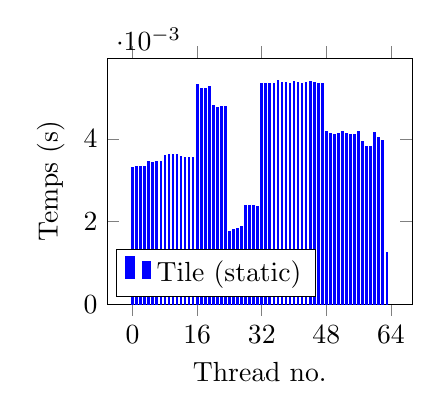
\begin{tikzpicture}
\begin{axis}[
  ybar,
  bar width=0.02cm,
  xlabel={Thread no.},
  ylabel={Temps (s)},
  ymin=0,
  legend pos=south west,
  width=0.45\textwidth,
  xtick distance=16
]

% Données pour le premier graphique (à gauche)
\addplot[color=blue, fill=blue] coordinates {
  (0,0.003311) (1,0.003324) (2,0.003322) (3,0.003336) (4,0.003450) (5,0.003439) (6,0.003442) (7,0.003460) (8,0.003596) (9,0.003616) (10,0.003627) (11,0.003630) (12,0.003580) (13,0.003553) (14,0.003544) (15,0.003558) (16,0.005311) (17,0.005224) (18,0.005222) (19,0.005270) (20,0.004809) (21,0.004762) (22,0.004773) (23,0.004789) (24,0.001770) (25,0.001799) (26,0.001824) (27,0.001871) (28,0.002395) (29,0.002378) (30,0.002379) (31,0.002375) (32,0.005344) (33,0.005338) (34,0.005350) (35,0.005350) (36,0.005415) (37,0.005367) (38,0.005358) (39,0.005341) (40,0.005390) (41,0.005356) (42,0.005331) (43,0.005363) (44,0.005389) (45,0.005373) (46,0.005352) (47,0.005350) (48,0.004174) (49,0.004142) (50,0.004118) (51,0.004130) (52,0.004184) (53,0.004140) (54,0.004095) (55,0.004117) (56,0.004169) (57,0.003949) (58,0.003828) (59,0.003806) (60,0.004147) (61,0.004036) (62,0.003970) (63,0.001240)
};
\addlegendentry{Tile (static)}

\end{axis}
\end{tikzpicture}
\hfill
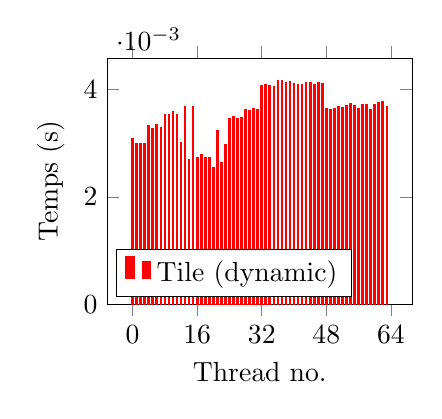
\begin{tikzpicture}
\begin{axis}[
  ybar,
  bar width=0.02cm,
  xlabel={Thread no.},
  ylabel={Temps (s)},
  ymin=0,
  legend pos=south west,
  width=0.45\textwidth,
  xtick distance=16
]

% Données pour le deuxième graphique (au milieu)
\addplot[color=red, fill=red] coordinates {
  (0,0.003094) (1,0.002995) (2,0.002995) (3,0.002989) (4,0.003326) (5,0.003271) (6,0.003353) (7,0.003304) (8,0.003542) (9,0.003539) (10,0.003594) (11,0.003545) (12,0.003022) (13,0.003678) (14,0.002699) (15,0.003696) (16,0.002738) (17,0.002794) (18,0.002728) (19,0.002735) (20,0.002557) (21,0.003236) (22,0.002643) (23,0.002973) (24,0.003458) (25,0.003493) (26,0.003468) (27,0.003477) (28,0.003624) (29,0.003603) (30,0.003652) (31,0.003625) (32,0.004086) (33,0.004100) (34,0.004085) (35,0.004060) (36,0.004170) (37,0.004173) (38,0.004134) (39,0.004148) (40,0.004119) (41,0.004106) (42,0.004099) (43,0.004134) (44,0.004136) (45,0.004103) (46,0.004126) (47,0.004118) (48,0.003646) (49,0.003631) (50,0.003655) (51,0.003680) (52,0.003664) (53,0.003698) (54,0.003745) (55,0.003707) (56,0.003649) (57,0.003723) (58,0.003722) (59,0.003636) (60,0.003733) (61,0.003760) (62,0.003786) (63,0.003681)
};
\addlegendentry{Tile (dynamic)}

\end{axis}
\end{tikzpicture}
\hfill
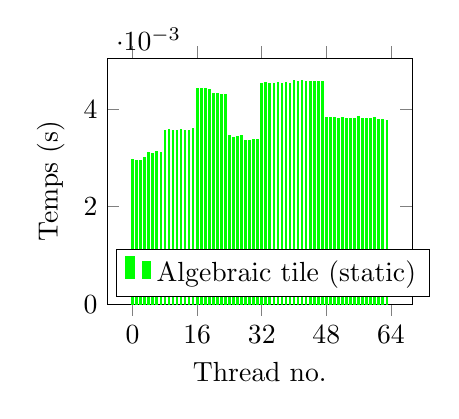
\begin{tikzpicture}
\begin{axis}[
  ybar,
  bar width=0.02cm,
  xlabel={Thread no.},
  ylabel={Temps (s)},
  ymin=0,
  legend pos=south west,
  width=0.45\textwidth,
  xtick distance=16
]

% Données pour le troisième graphique (à droite)
\addplot[color=green, fill=green] coordinates {
  (0,0.002963) (1,0.002956) (2,0.002959) (3,0.003006) (4,0.003118) (5,0.003097) (6,0.003124) (7,0.003110) (8,0.003572) (9,0.003592) (10,0.003567) (11,0.003565) (12,0.003584) (13,0.003558) (14,0.003562) (15,0.003600) (16,0.004428) (17,0.004428) (18,0.004431) (19,0.004416) (20,0.004315) (21,0.004329) (22,0.004308) (23,0.004314) (24,0.003458) (25,0.003422) (26,0.003438) (27,0.003456) (28,0.003358) (29,0.003366) (30,0.003387) (31,0.003374) (32,0.004535) (33,0.004545) (34,0.004538) (35,0.004525) (36,0.004560) (37,0.004528) (38,0.004547) (39,0.004528) (40,0.004593) (41,0.004575) (42,0.004586) (43,0.004569) (44,0.004578) (45,0.004568) (46,0.004576) (47,0.004575) (48,0.003830) (49,0.003830) (50,0.003828) (51,0.003818) (52,0.003841) (53,0.003807) (54,0.003807) (55,0.003810) (56,0.003847) (57,0.003802) (58,0.003817) (59,0.003815) (60,0.003822) (61,0.003789) (62,0.003782) (63,0.003780)
};
\addlegendentry{Algebraic tile (static)}

\end{axis}
\end{tikzpicture}

\caption{Temps d'exécution des threads pour le fichier gesummv.c}
\label{fig:graphes}
\end{figure}

\begin{table}[htbp]
  \centering
  \caption{Statistiques pour le fichier gesummv.c}
  \begin{tabular}{|c|c|c|c|}
    \hline
    Statistique & Algebraic Tile & Tile (static) & Tile (dynamic) \\ 
    \hline
    Skewness (g1)  & -0.0635151 & -0.557278 & -0.553388 \\ 
    Kurtosis (g2)  & -1.23563 & -0.428484 & -0.535031 \\ 
    Coefficient de variation $ \frac{\sigma}{\overline{x}} $ & 0.134683 & 0.274283 & 0.125271\\ 
    Percent Imbalance metric en \% & 18.0001 & 32.9085 & 16.9016\\ 
    Coefficient de Gini  & 0.0760475 & 0.151832 & 0.06953\\ 
    Temps d'exécution (s) &  0.004694    &  0.005546   &  0.004320   \\ 

    \hline
  \end{tabular}
\end{table}
g1=$ \frac{\sum_{i=1}^{n} (x_i - \overline{x})^3}{n\sigma^3} $\
g2=$ \frac{\sum_{i=1}^{n} (x_i - \overline{x})^4}{n\sigma^4} $\
Coefficient de Gini = $ \frac{\sum_{i=1}^{n}\sum_{j=1}^{n} |x_i - x_j|}{2n^2\overline{x}} $\
\newpage

\begin{figure}
\centering

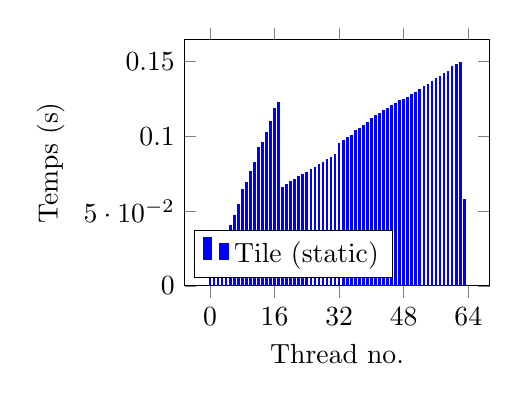
\begin{tikzpicture}
\begin{axis}[
  ybar,
  bar width=0.02cm,
  xlabel={Thread no.},
  ylabel={Temps (s)},
  ymin=0,
  legend pos=south west,
  width=0.45\textwidth,
  xtick distance=16
]

% Données pour le premier graphique (à gauche)
\addplot[color=blue, fill=blue] coordinates {
  (0,0.004876) (1,0.011706) (2,0.019011) (3,0.026133) (4,0.034385) (5,0.040539) (6,0.047234) (7,0.054044) (8,0.064399) (9,0.068941) (10,0.076312) (11,0.082637) (12,0.092105) (13,0.095641) (14,0.102737) (15,0.109530) (16,0.118725) (17,0.122182) (18,0.065916) (19,0.067640) (20,0.069740) (21,0.071234) (22,0.072858) (23,0.074490) (24,0.075927) (25,0.077511) (26,0.079120) (27,0.080736) (28,0.082706) (29,0.084303) (30,0.085896) (31,0.087494) (32,0.095377) (33,0.097146) (34,0.098914) (35,0.100672) (36,0.103605) (37,0.105315) (38,0.107023) (39,0.108815) (40,0.112001) (41,0.113621) (42,0.115230) (43,0.116836) (44,0.118757) (45,0.120319) (46,0.121912) (47,0.123522) (48,0.124493) (49,0.126150) (50,0.127778) (51,0.129394) (52,0.131424) (53,0.132997) (54,0.134585) (55,0.136199) (56,0.138560) (57,0.140148) (58,0.141759) (59,0.143407) (60,0.146242) (61,0.147842) (62,0.149497) (63,0.057928)
};
\addlegendentry{Tile (static)}

\end{axis}
\end{tikzpicture}
\hfill
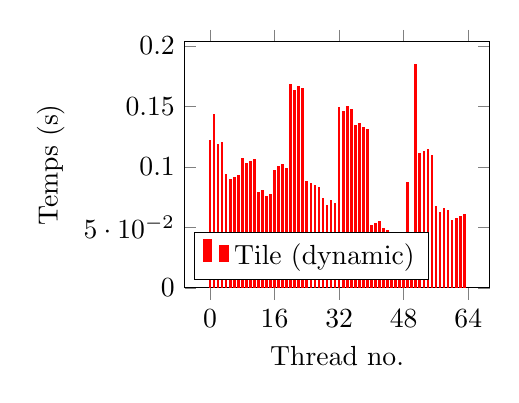
\begin{tikzpicture}
\begin{axis}[
  ybar,
  bar width=0.02cm,
  xlabel={Thread no.},
  ylabel={Temps (s)},
  ymin=0,
  legend pos=south west,
  width=0.45\textwidth,
  xtick distance=16
]

% Données pour le deuxième graphique (au milieu)
\addplot[color=red, fill=red] coordinates {
  (0,0.121908) (1,0.143020) (2,0.118656) (3,0.120196) (4,0.093966) (5,0.089345) (6,0.090771) (7,0.092399) (8,0.107060) (9,0.102572) (10,0.104203) (11,0.105830) (12,0.078859) (13,0.080409) (14,0.075508) (15,0.076957) (16,0.096943) (17,0.100115) (18,0.101708) (19,0.098527) (20,0.168008) (21,0.163184) (22,0.166393) (23,0.164794) (24,0.087476) (25,0.085829) (26,0.084129) (27,0.082450) (28,0.073561) (29,0.068186) (30,0.071762) (31,0.069958) (32,0.148562) (33,0.145371) (34,0.150183) (35,0.146972) (36,0.133811) (37,0.135423) (38,0.132205) (39,0.130585) (40,0.051061) (41,0.052771) (42,0.054456) (43,0.049357) (44,0.047048) (45,0.045348) (46,0.043572) (47,0.041814) (48,0.036775) (49,0.086693) (50,0.038585) (51,0.184872) (52,0.111047) (53,0.112610) (54,0.114299) (55,0.109363) (56,0.066999) (57,0.062236) (58,0.065404) (59,0.063842) (60,0.055485) (61,0.056960) (62,0.058814) (63,0.060427)
};
\addlegendentry{Tile (dynamic)}

\end{axis}
\end{tikzpicture}
\hfill
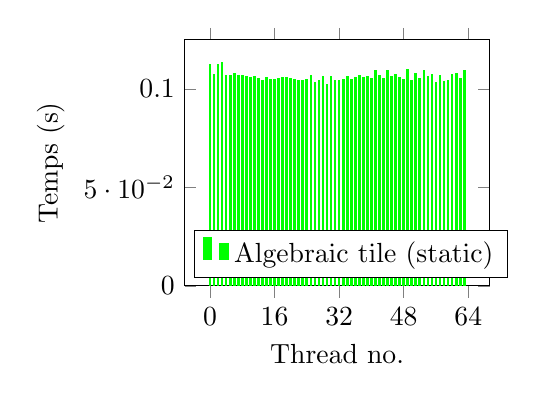
\begin{tikzpicture}
\begin{axis}[
  ybar,
  bar width=0.02cm,
  xlabel={Thread no.},
  ylabel={Temps (s)},
  ymin=0,
  legend pos=south west,
  width=0.45\textwidth,
  xtick distance=16
]

% Données pour le troisième graphique (à droite)
\addplot[color=green, fill=green] coordinates {
  (0,0.112240) (1,0.107279) (2,0.112349) (3,0.113671) (4,0.107009) (5,0.106648) (6,0.107756) (7,0.106649) (8,0.106744) (9,0.106381) (10,0.106050) (11,0.106311) (12,0.105180) (13,0.104446) (14,0.105674) (15,0.104756) (16,0.105054) (17,0.105430) (18,0.105675) (19,0.105681) (20,0.105237) (21,0.104634) (22,0.104345) (23,0.104246) (24,0.104937) (25,0.106902) (26,0.103301) (27,0.104214) (28,0.106139) (29,0.102087) (30,0.106282) (31,0.104449) (32,0.104556) (33,0.104940) (34,0.106227) (35,0.104979) (36,0.105938) (37,0.106796) (38,0.105883) (39,0.106124) (40,0.105460) (41,0.109530) (42,0.106900) (43,0.105441) (44,0.109470) (45,0.106112) (46,0.107297) (47,0.105746) (48,0.104938) (49,0.109927) (50,0.104159) (51,0.108117) (52,0.105500) (53,0.109447) (54,0.106264) (55,0.107133) (56,0.103335) (57,0.107092) (58,0.103722) (59,0.104372) (60,0.107376) (61,0.107632) (62,0.105333) (63,0.109324)
};
\addlegendentry{Algebraic tile (static)}

\end{axis}
\end{tikzpicture}

\caption{Temps d'exécution des threads pour le fichier syr2k.c}
\label{fig:graphes}
\end{figure}

\begin{table}[htbp]
  \centering
  \caption{Statistiques pour le fichier syr2k.c}
  \begin{tabular}{|c|c|c|c|}
    \hline
    Statistique & Algebraic Tile & Tile (static) & Tile (dynamic) \\ 
    \hline
    Skewness (g1)  & 1.30264 & -0.598581 & 0.463089 \\ 
    Kurtosis (g2)  & 2.2822 & -0.198786 & -0.649789 \\ 
    Coefficient de variation $ \frac{\sigma}{\overline{x}} $ & 0.019934 & 0.366102 & 0.391293\\ 
    Percent Imbalance metric en \% & 6.94018 & 56.4856 & 94.6779\\ 
    Coefficient de Gini  & 0.0103782 & 0.20571 & 0.222297\\ 
    Temps d'exécution (s) &  0.114699    &  0.149728   &  0.185561   \\ 

    \hline
  \end{tabular}
\end{table}
g1=$ \frac{\sum_{i=1}^{n} (x_i - \overline{x})^3}{n\sigma^3} $\
g2=$ \frac{\sum_{i=1}^{n} (x_i - \overline{x})^4}{n\sigma^4} $\
Coefficient de Gini = $ \frac{\sum_{i=1}^{n}\sum_{j=1}^{n} |x_i - x_j|}{2n^2\overline{x}} $\
\newpage

\begin{figure}
\centering

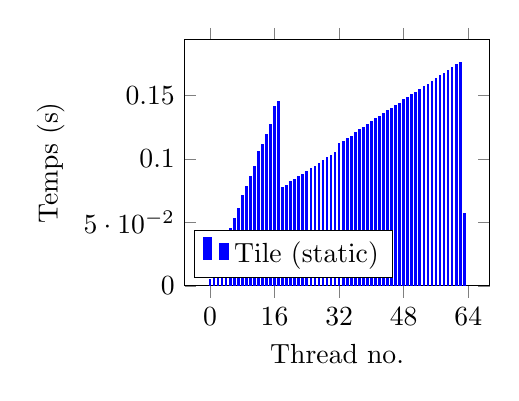
\begin{tikzpicture}
\begin{axis}[
  ybar,
  bar width=0.02cm,
  xlabel={Thread no.},
  ylabel={Temps (s)},
  ymin=0,
  legend pos=south west,
  width=0.45\textwidth,
  xtick distance=16
]

% Données pour le premier graphique (à gauche)
\addplot[color=blue, fill=blue] coordinates {
  (0,0.004655) (1,0.012422) (2,0.020472) (3,0.028383) (4,0.037099) (5,0.044971) (6,0.052914) (7,0.060830) (8,0.070869) (9,0.078159) (10,0.085984) (11,0.093979) (12,0.106055) (13,0.111049) (14,0.118961) (15,0.127176) (16,0.141133) (17,0.145253) (18,0.077099) (19,0.079095) (20,0.081973) (21,0.083938) (22,0.085941) (23,0.087932) (24,0.090222) (25,0.092227) (26,0.094232) (27,0.096204) (28,0.099028) (29,0.100988) (30,0.102977) (31,0.105197) (32,0.111928) (33,0.113879) (34,0.115863) (35,0.117872) (36,0.121101) (37,0.123065) (38,0.125046) (39,0.127038) (40,0.129556) (41,0.131542) (42,0.133519) (43,0.135500) (44,0.137901) (45,0.139879) (46,0.141858) (47,0.143836) (48,0.146618) (49,0.148579) (50,0.150564) (51,0.152537) (52,0.155161) (53,0.157123) (54,0.159119) (55,0.161105) (56,0.163818) (57,0.165807) (58,0.167785) (59,0.169774) (60,0.172475) (61,0.174485) (62,0.176435) (63,0.057242)
};
\addlegendentry{Tile (static)}

\end{axis}
\end{tikzpicture}
\hfill
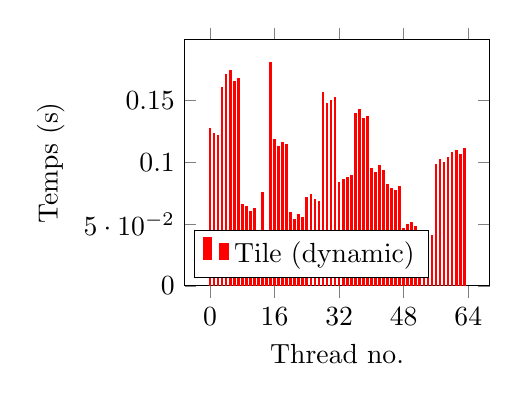
\begin{tikzpicture}
\begin{axis}[
  ybar,
  bar width=0.02cm,
  xlabel={Thread no.},
  ylabel={Temps (s)},
  ymin=0,
  legend pos=south west,
  width=0.45\textwidth,
  xtick distance=16
]

% Données pour le deuxième graphique (au milieu)
\addplot[color=red, fill=red] coordinates {
  (0,0.127417) (1,0.123151) (2,0.121413) (3,0.160596) (4,0.170814) (5,0.174510) (6,0.165722) (7,0.167536) (8,0.065829) (9,0.064013) (10,0.060383) (11,0.062269) (12,0.036570) (13,0.075588) (14,0.034750) (15,0.181165) (16,0.118226) (17,0.112761) (18,0.116399) (19,0.114566) (20,0.059133) (21,0.053692) (22,0.057314) (23,0.055490) (24,0.071666) (25,0.073500) (26,0.069841) (27,0.068038) (28,0.156189) (29,0.147960) (30,0.149763) (31,0.152604) (32,0.083854) (33,0.085724) (34,0.087551) (35,0.089459) (36,0.139266) (37,0.143007) (38,0.135569) (39,0.137395) (40,0.095237) (41,0.091541) (42,0.097050) (43,0.093349) (44,0.082204) (45,0.078571) (46,0.076752) (47,0.080383) (48,0.046126) (49,0.049765) (50,0.051557) (51,0.048006) (52,0.044194) (53,0.042648) (54,0.038750) (55,0.040822) (56,0.098321) (57,0.102016) (58,0.100114) (59,0.103915) (60,0.107837) (61,0.109661) (62,0.106038) (63,0.111491)
};
\addlegendentry{Tile (dynamic)}

\end{axis}
\end{tikzpicture}
\hfill
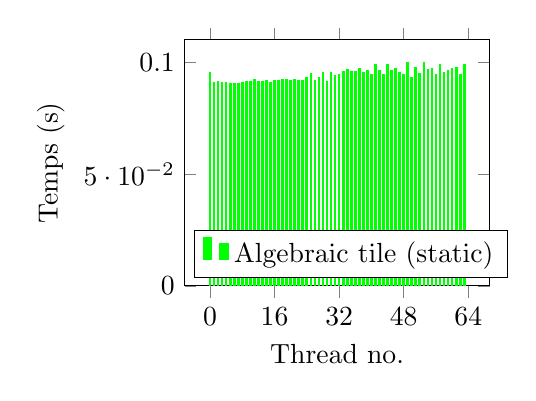
\begin{tikzpicture}
\begin{axis}[
  ybar,
  bar width=0.02cm,
  xlabel={Thread no.},
  ylabel={Temps (s)},
  ymin=0,
  legend pos=south west,
  width=0.45\textwidth,
  xtick distance=16
]

% Données pour le troisième graphique (à droite)
\addplot[color=green, fill=green] coordinates {
  (0,0.095400) (1,0.091083) (2,0.091490) (3,0.091000) (4,0.090841) (5,0.090432) (6,0.090634) (7,0.090445) (8,0.090920) (9,0.091383) (10,0.091259) (11,0.092182) (12,0.091169) (13,0.091270) (14,0.091596) (15,0.090970) (16,0.091584) (17,0.091828) (18,0.092357) (19,0.092217) (20,0.091932) (21,0.092386) (22,0.091641) (23,0.091571) (24,0.093225) (25,0.094978) (26,0.091759) (27,0.092908) (28,0.095344) (29,0.091210) (30,0.095158) (31,0.094114) (32,0.094456) (33,0.095584) (34,0.096636) (35,0.095695) (36,0.095696) (37,0.097155) (38,0.095547) (39,0.096204) (40,0.094527) (41,0.099147) (42,0.096365) (43,0.094534) (44,0.098866) (45,0.096076) (46,0.097200) (47,0.095136) (48,0.094676) (49,0.100011) (50,0.093317) (51,0.097631) (52,0.094907) (53,0.099703) (54,0.096569) (55,0.097201) (56,0.094335) (57,0.099008) (58,0.095422) (59,0.096110) (60,0.097006) (61,0.097664) (62,0.094598) (63,0.099024)
};
\addlegendentry{Algebraic tile (static)}

\end{axis}
\end{tikzpicture}

\caption{Temps d'exécution des threads pour le fichier syrk.c}
\label{fig:graphes}
\end{figure}

\begin{table}[htbp]
  \centering
  \caption{Statistiques pour le fichier syrk.c}
  \begin{tabular}{|c|c|c|c|}
    \hline
    Statistique & Algebraic Tile & Tile (static) & Tile (dynamic) \\ 
    \hline
    Skewness (g1)  & 0.307614 & -0.589556 & 0.37718 \\ 
    Kurtosis (g2)  & -1.00175 & -0.234098 & -0.849964 \\ 
    Coefficient de variation $ \frac{\sigma}{\overline{x}} $ & 0.028577 & 0.376141 & 0.411815\\ 
    Percent Imbalance metric en \% & 6.10729 & 58.0293 & 88.0085\\ 
    Coefficient de Gini  & 0.0162455 & 0.211556 & 0.235193\\ 
    Temps d'exécution (s) &  0.100436    &  0.176745   &  0.182015   \\ 

    \hline
  \end{tabular}
\end{table}
g1=$ \frac{\sum_{i=1}^{n} (x_i - \overline{x})^3}{n\sigma^3} $\
g2=$ \frac{\sum_{i=1}^{n} (x_i - \overline{x})^4}{n\sigma^4} $\
Coefficient de Gini = $ \frac{\sum_{i=1}^{n}\sum_{j=1}^{n} |x_i - x_j|}{2n^2\overline{x}} $\
\newpage

\begin{figure}
\centering

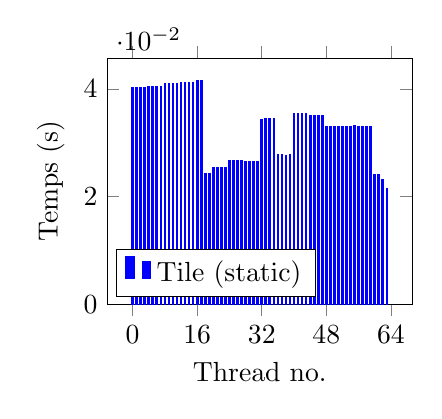
\begin{tikzpicture}
\begin{axis}[
  ybar,
  bar width=0.02cm,
  xlabel={Thread no.},
  ylabel={Temps (s)},
  ymin=0,
  legend pos=south west,
  width=0.45\textwidth,
  xtick distance=16
]

% Données pour le premier graphique (à gauche)
\addplot[color=blue, fill=blue] coordinates {
  (0,0.040198) (1,0.040166) (2,0.040172) (3,0.040239) (4,0.040449) (5,0.040429) (6,0.040440) (7,0.040436) (8,0.040998) (9,0.041024) (10,0.041011) (11,0.041027) (12,0.041155) (13,0.041113) (14,0.041124) (15,0.041239) (16,0.041543) (17,0.041557) (18,0.024243) (19,0.024234) (20,0.025359) (21,0.025356) (22,0.025369) (23,0.025365) (24,0.026625) (25,0.026617) (26,0.026673) (27,0.026632) (28,0.026482) (29,0.026436) (30,0.026431) (31,0.026487) (32,0.034383) (33,0.034411) (34,0.034412) (35,0.034395) (36,0.027722) (37,0.027711) (38,0.027694) (39,0.027723) (40,0.035505) (41,0.035491) (42,0.035505) (43,0.035503) (44,0.034992) (45,0.034983) (46,0.034976) (47,0.034986) (48,0.032932) (49,0.032948) (50,0.032961) (51,0.032941) (52,0.033076) (53,0.033027) (54,0.033041) (55,0.033127) (56,0.033070) (57,0.033078) (58,0.033077) (59,0.033034) (60,0.024087) (61,0.024022) (62,0.023157) (63,0.021409)
};
\addlegendentry{Tile (static)}

\end{axis}
\end{tikzpicture}
\hfill
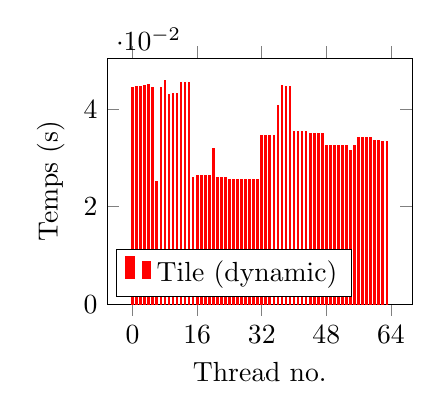
\begin{tikzpicture}
\begin{axis}[
  ybar,
  bar width=0.02cm,
  xlabel={Thread no.},
  ylabel={Temps (s)},
  ymin=0,
  legend pos=south west,
  width=0.45\textwidth,
  xtick distance=16
]

% Données pour le deuxième graphique (au milieu)
\addplot[color=red, fill=red] coordinates {
  (0,0.044335) (1,0.044600) (2,0.044642) (3,0.044749) (4,0.045043) (5,0.044337) (6,0.025132) (7,0.044354) (8,0.045863) (9,0.043080) (10,0.043103) (11,0.043096) (12,0.045419) (13,0.045521) (14,0.045407) (15,0.025904) (16,0.026392) (17,0.026376) (18,0.026410) (19,0.026371) (20,0.031814) (21,0.026024) (22,0.026022) (23,0.025894) (24,0.025588) (25,0.025598) (26,0.025565) (27,0.025630) (28,0.025605) (29,0.025572) (30,0.025578) (31,0.025604) (32,0.034553) (33,0.034547) (34,0.034567) (35,0.034566) (36,0.040665) (37,0.044764) (38,0.044639) (39,0.044668) (40,0.035466) (41,0.035445) (42,0.035462) (43,0.035445) (44,0.034915) (45,0.034920) (46,0.034921) (47,0.034922) (48,0.032466) (49,0.032457) (50,0.032474) (51,0.032468) (52,0.032457) (53,0.032442) (54,0.031472) (55,0.032468) (56,0.034194) (57,0.034203) (58,0.034203) (59,0.034220) (60,0.033476) (61,0.033483) (62,0.033417) (63,0.033319)
};
\addlegendentry{Tile (dynamic)}

\end{axis}
\end{tikzpicture}
\hfill
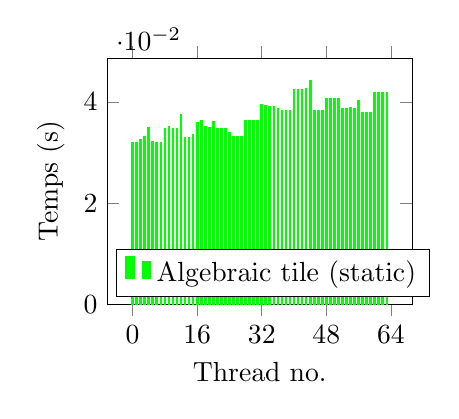
\begin{tikzpicture}
\begin{axis}[
  ybar,
  bar width=0.02cm,
  xlabel={Thread no.},
  ylabel={Temps (s)},
  ymin=0,
  legend pos=south west,
  width=0.45\textwidth,
  xtick distance=16
]

% Données pour le troisième graphique (à droite)
\addplot[color=green, fill=green] coordinates {
  (0,0.032045) (1,0.031999) (2,0.032486) (3,0.033079) (4,0.034934) (5,0.032130) (6,0.032029) (7,0.032049) (8,0.034768) (9,0.035251) (10,0.034758) (11,0.034765) (12,0.037569) (13,0.032895) (14,0.032914) (15,0.033629) (16,0.035891) (17,0.036436) (18,0.035114) (19,0.035055) (20,0.036172) (21,0.034791) (22,0.034782) (23,0.034767) (24,0.034020) (25,0.033193) (26,0.033181) (27,0.033180) (28,0.036398) (29,0.036342) (30,0.036363) (31,0.036379) (32,0.039513) (33,0.039309) (34,0.039132) (35,0.039061) (36,0.038682) (37,0.038269) (38,0.038281) (39,0.038280) (40,0.042483) (41,0.042496) (42,0.042496) (43,0.042683) (44,0.044271) (45,0.038370) (46,0.038373) (47,0.038367) (48,0.040781) (49,0.040711) (50,0.040693) (51,0.040754) (52,0.038785) (53,0.038725) (54,0.038821) (55,0.038807) (56,0.040315) (57,0.037884) (58,0.037881) (59,0.037883) (60,0.041882) (61,0.041847) (62,0.041875) (63,0.041854)
};
\addlegendentry{Algebraic tile (static)}

\end{axis}
\end{tikzpicture}

\caption{Temps d'exécution des threads pour le fichier trmm.c}
\label{fig:graphes}
\end{figure}

\begin{table}[htbp]
  \centering
  \caption{Statistiques pour le fichier trmm.c}
  \begin{tabular}{|c|c|c|c|}
    \hline
    Statistique & Algebraic Tile & Tile (static) & Tile (dynamic) \\ 
    \hline
    Skewness (g1)  & 0.125044 & -0.106473 & 0.24028 \\ 
    Kurtosis (g2)  & -0.996617 & -1.27733 & -1.16723 \\ 
    Coefficient de variation $ \frac{\sigma}{\overline{x}} $ & 0.0882324 & 0.184024 & 0.200861\\ 
    Percent Imbalance metric en \% & 19.1016 & 25.6919 & 32.3184\\ 
    Coefficient de Gini  & 0.0505529 & 0.10414 & 0.112078\\ 
    Temps d'exécution (s) &  0.044568    &  0.043292   &  0.047441   \\ 

    \hline
  \end{tabular}
\end{table}
g1=$ \frac{\sum_{i=1}^{n} (x_i - \overline{x})^3}{n\sigma^3} $\
g2=$ \frac{\sum_{i=1}^{n} (x_i - \overline{x})^4}{n\sigma^4} $\
Coefficient de Gini = $ \frac{\sum_{i=1}^{n}\sum_{j=1}^{n} |x_i - x_j|}{2n^2\overline{x}} $\
\newpage

\begin{figure}
\centering

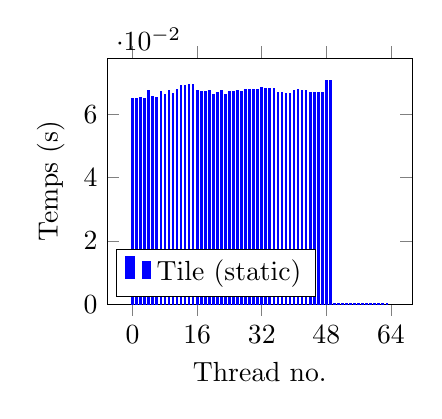
\begin{tikzpicture}
\begin{axis}[
  ybar,
  bar width=0.02cm,
  xlabel={Thread no.},
  ylabel={Temps (s)},
  ymin=0,
  legend pos=south west,
  width=0.45\textwidth,
  xtick distance=16
]

% Données pour le premier graphique (à gauche)
\addplot[color=blue, fill=blue] coordinates {
  (0,0.065084) (1,0.065088) (2,0.065185) (3,0.065103) (4,0.067533) (5,0.065462) (6,0.065360) (7,0.067244) (8,0.066132) (9,0.067419) (10,0.066548) (11,0.067742) (12,0.069137) (13,0.069168) (14,0.069250) (15,0.069245) (16,0.067439) (17,0.067078) (18,0.067025) (19,0.067442) (20,0.066253) (21,0.066956) (22,0.067448) (23,0.066259) (24,0.067241) (25,0.067301) (26,0.067336) (27,0.067204) (28,0.067755) (29,0.067710) (30,0.067856) (31,0.067942) (32,0.068319) (33,0.068256) (34,0.068259) (35,0.068153) (36,0.066718) (37,0.066750) (38,0.066666) (39,0.066615) (40,0.067630) (41,0.067663) (42,0.067639) (43,0.067606) (44,0.066830) (45,0.066965) (46,0.066800) (47,0.066890) (48,0.070661) (49,0.070665) (50,0.000051) (51,0.000051) (52,0.000051) (53,0.000051) (54,0.000051) (55,0.000051) (56,0.000052) (57,0.000052) (58,0.000052) (59,0.000052) (60,0.000053) (61,0.000053) (62,0.000053) (63,0.000053)
};
\addlegendentry{Tile (static)}

\end{axis}
\end{tikzpicture}
\hfill
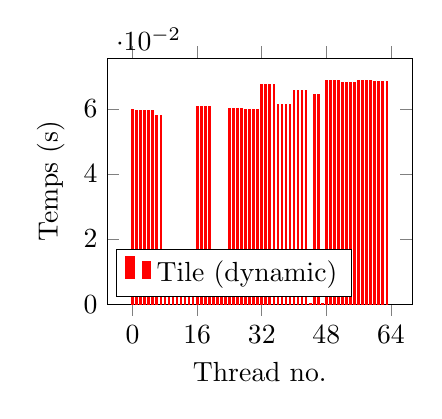
\begin{tikzpicture}
\begin{axis}[
  ybar,
  bar width=0.02cm,
  xlabel={Thread no.},
  ylabel={Temps (s)},
  ymin=0,
  legend pos=south west,
  width=0.45\textwidth,
  xtick distance=16
]

% Données pour le deuxième graphique (au milieu)
\addplot[color=red, fill=red] coordinates {
  (0,0.059700) (1,0.059471) (2,0.059503) (3,0.059526) (4,0.059321) (5,0.059364) (6,0.057866) (7,0.057872) (8,0.002452) (9,0.002456) (10,0.002443) (11,0.002479) (12,0.002449) (13,0.002437) (14,0.002448) (15,0.002424) (16,0.060682) (17,0.060693) (18,0.060691) (19,0.060703) (20,0.002758) (21,0.002752) (22,0.002712) (23,0.002720) (24,0.059983) (25,0.060099) (26,0.059978) (27,0.059996) (28,0.059818) (29,0.059839) (30,0.059831) (31,0.059824) (32,0.067461) (33,0.067480) (34,0.067542) (35,0.067455) (36,0.061293) (37,0.061293) (38,0.061297) (39,0.061300) (40,0.065659) (41,0.065657) (42,0.065657) (43,0.065663) (44,0.000074) (45,0.064341) (46,0.064332) (47,0.000075) (48,0.068555) (49,0.068554) (50,0.068557) (51,0.068572) (52,0.068051) (53,0.068016) (54,0.068041) (55,0.068022) (56,0.068697) (57,0.068699) (58,0.068703) (59,0.068685) (60,0.068306) (61,0.068246) (62,0.068249) (63,0.068297)
};
\addlegendentry{Tile (dynamic)}

\end{axis}
\end{tikzpicture}
\hfill
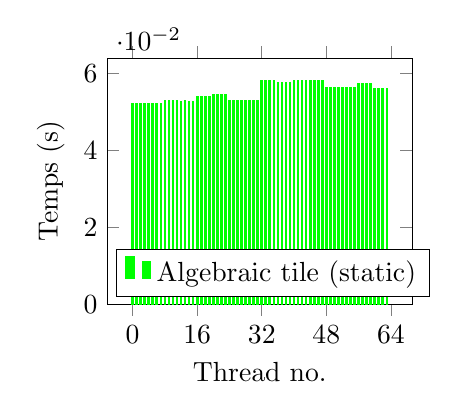
\begin{tikzpicture}
\begin{axis}[
  ybar,
  bar width=0.02cm,
  xlabel={Thread no.},
  ylabel={Temps (s)},
  ymin=0,
  legend pos=south west,
  width=0.45\textwidth,
  xtick distance=16
]

% Données pour le troisième graphique (à droite)
\addplot[color=green, fill=green] coordinates {
  (0,0.052157) (1,0.052191) (2,0.052205) (3,0.052198) (4,0.052175) (5,0.052178) (6,0.052207) (7,0.052179) (8,0.052879) (9,0.052913) (10,0.052873) (11,0.052872) (12,0.052756) (13,0.052837) (14,0.052753) (15,0.052772) (16,0.053923) (17,0.053900) (18,0.053916) (19,0.053915) (20,0.054378) (21,0.054360) (22,0.054352) (23,0.054391) (24,0.052960) (25,0.052962) (26,0.052958) (27,0.052956) (28,0.052949) (29,0.052965) (30,0.052976) (31,0.052929) (32,0.058021) (33,0.058012) (34,0.058003) (35,0.057976) (36,0.057632) (37,0.057631) (38,0.057631) (39,0.057676) (40,0.058084) (41,0.058087) (42,0.058093) (43,0.058067) (44,0.058120) (45,0.058115) (46,0.058113) (47,0.058102) (48,0.056172) (49,0.056205) (50,0.056189) (51,0.056206) (52,0.056270) (53,0.056274) (54,0.056258) (55,0.056262) (56,0.057255) (57,0.057285) (58,0.057283) (59,0.057282) (60,0.056124) (61,0.056124) (62,0.056139) (63,0.056094)
};
\addlegendentry{Algebraic tile (static)}

\end{axis}
\end{tikzpicture}

\caption{Temps d'exécution des threads pour le fichier 2mm.c}
\label{fig:graphes}
\end{figure}

\begin{table}[htbp]
  \centering
  \caption{Statistiques pour le fichier 2mm.c}
  \begin{tabular}{|c|c|c|c|}
    \hline
    Statistique & Algebraic Tile & Tile (static) & Tile (dynamic) \\ 
    \hline
    Skewness (g1)  & 0.0535635 & -1.35513 & -1.29597 \\ 
    Kurtosis (g2)  & -1.63119 & -0.154612 & -0.216938 \\ 
    Coefficient de variation $ \frac{\sigma}{\overline{x}} $ & 0.0404635 & 0.529031 & 0.510884\\ 
    Percent Imbalance metric en \% & 5.44152 & 34.3298 & 36.2936\\ 
    Coefficient de Gini  & 0.0227733 & 0.226241 & 0.235915\\ 
    Temps d'exécution (s) &  0.058643    &  0.071928   &  0.068823   \\ 

    \hline
  \end{tabular}
\end{table}
g1=$ \frac{\sum_{i=1}^{n} (x_i - \overline{x})^3}{n\sigma^3} $\
g2=$ \frac{\sum_{i=1}^{n} (x_i - \overline{x})^4}{n\sigma^4} $\
Coefficient de Gini = $ \frac{\sum_{i=1}^{n}\sum_{j=1}^{n} |x_i - x_j|}{2n^2\overline{x}} $\
\newpage

\begin{figure}
\centering

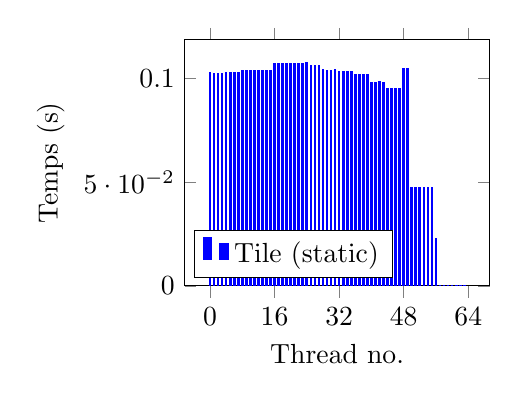
\begin{tikzpicture}
\begin{axis}[
  ybar,
  bar width=0.02cm,
  xlabel={Thread no.},
  ylabel={Temps (s)},
  ymin=0,
  legend pos=south west,
  width=0.45\textwidth,
  xtick distance=16
]

% Données pour le premier graphique (à gauche)
\addplot[color=blue, fill=blue] coordinates {
  (0,0.102510) (1,0.102368) (2,0.102237) (3,0.102224) (4,0.102454) (5,0.102476) (6,0.102453) (7,0.102435) (8,0.103531) (9,0.103546) (10,0.103522) (11,0.103515) (12,0.103442) (13,0.103494) (14,0.103428) (15,0.103474) (16,0.106868) (17,0.106807) (18,0.106804) (19,0.106842) (20,0.107108) (21,0.107096) (22,0.107125) (23,0.107122) (24,0.107687) (25,0.106151) (26,0.106107) (27,0.106113) (28,0.104067) (29,0.103858) (30,0.103841) (31,0.103883) (32,0.103320) (33,0.103315) (34,0.103320) (35,0.103280) (36,0.101891) (37,0.101882) (38,0.101883) (39,0.101888) (40,0.098058) (41,0.098071) (42,0.098094) (43,0.098077) (44,0.094783) (45,0.094782) (46,0.094786) (47,0.094789) (48,0.104821) (49,0.104833) (50,0.047326) (51,0.047326) (52,0.047370) (53,0.047353) (54,0.047353) (55,0.047353) (56,0.022722) (57,0.000101) (58,0.000100) (59,0.000101) (60,0.000100) (61,0.000100) (62,0.000100) (63,0.000100)
};
\addlegendentry{Tile (static)}

\end{axis}
\end{tikzpicture}
\hfill
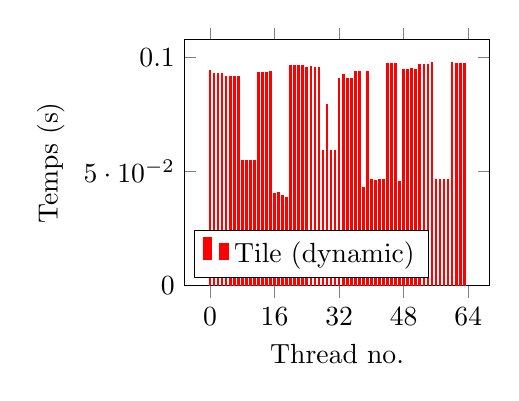
\begin{tikzpicture}
\begin{axis}[
  ybar,
  bar width=0.02cm,
  xlabel={Thread no.},
  ylabel={Temps (s)},
  ymin=0,
  legend pos=south west,
  width=0.45\textwidth,
  xtick distance=16
]

% Données pour le deuxième graphique (au milieu)
\addplot[color=red, fill=red] coordinates {
  (0,0.094035) (1,0.093031) (2,0.093080) (3,0.093041) (4,0.091801) (5,0.091656) (6,0.091614) (7,0.091658) (8,0.054617) (9,0.054635) (10,0.054637) (11,0.054621) (12,0.093154) (13,0.093205) (14,0.093154) (15,0.093557) (16,0.040191) (17,0.040850) (18,0.039607) (19,0.038567) (20,0.096219) (21,0.096240) (22,0.096236) (23,0.096219) (24,0.095612) (25,0.095756) (26,0.095623) (27,0.095621) (28,0.059087) (29,0.079409) (30,0.059053) (31,0.059082) (32,0.090847) (33,0.092390) (34,0.090864) (35,0.090835) (36,0.093589) (37,0.093615) (38,0.042818) (39,0.093635) (40,0.046288) (41,0.046277) (42,0.046315) (43,0.046316) (44,0.097368) (45,0.097410) (46,0.097384) (47,0.045530) (48,0.094623) (49,0.094674) (50,0.095096) (51,0.094695) (52,0.096978) (53,0.096965) (54,0.096986) (55,0.097607) (56,0.046529) (57,0.046517) (58,0.046531) (59,0.046523) (60,0.097899) (61,0.097250) (62,0.097125) (63,0.097185)
};
\addlegendentry{Tile (dynamic)}

\end{axis}
\end{tikzpicture}
\hfill
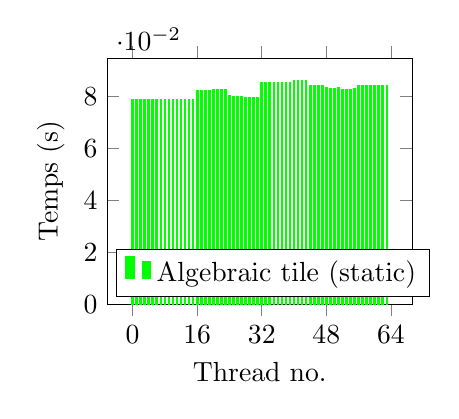
\begin{tikzpicture}
\begin{axis}[
  ybar,
  bar width=0.02cm,
  xlabel={Thread no.},
  ylabel={Temps (s)},
  ymin=0,
  legend pos=south west,
  width=0.45\textwidth,
  xtick distance=16
]

% Données pour le troisième graphique (à droite)
\addplot[color=green, fill=green] coordinates {
  (0,0.078727) (1,0.078744) (2,0.078759) (3,0.078795) (4,0.078759) (5,0.078762) (6,0.078764) (7,0.078755) (8,0.078900) (9,0.078890) (10,0.078879) (11,0.078856) (12,0.078803) (13,0.078823) (14,0.078771) (15,0.078771) (16,0.082299) (17,0.082287) (18,0.082264) (19,0.082287) (20,0.082628) (21,0.082591) (22,0.082606) (23,0.082649) (24,0.080084) (25,0.080073) (26,0.080055) (27,0.080040) (28,0.079641) (29,0.079594) (30,0.079576) (31,0.079598) (32,0.085249) (33,0.085240) (34,0.085200) (35,0.085127) (36,0.085180) (37,0.085206) (38,0.085176) (39,0.085208) (40,0.086030) (41,0.086059) (42,0.086057) (43,0.086058) (44,0.084211) (45,0.084285) (46,0.084253) (47,0.084280) (48,0.083181) (49,0.083143) (50,0.083146) (51,0.083155) (52,0.082730) (53,0.082735) (54,0.082716) (55,0.082800) (56,0.084217) (57,0.084209) (58,0.084177) (59,0.084188) (60,0.084269) (61,0.084275) (62,0.084255) (63,0.084301)
};
\addlegendentry{Algebraic tile (static)}

\end{axis}
\end{tikzpicture}

\caption{Temps d'exécution des threads pour le fichier 3mm.c}
\label{fig:graphes}
\end{figure}

\begin{table}[htbp]
  \centering
  \caption{Statistiques pour le fichier 3mm.c}
  \begin{tabular}{|c|c|c|c|}
    \hline
    Statistique & Algebraic Tile & Tile (static) & Tile (dynamic) \\ 
    \hline
    Skewness (g1)  & -0.150444 & -1.63565 & -0.77812 \\ 
    Kurtosis (g2)  & -1.48043 & 1.06218 & -1.24338 \\ 
    Coefficient de variation $ \frac{\sigma}{\overline{x}} $ & 0.0310795 & 0.413517 & 0.278411\\ 
    Percent Imbalance metric en \% & 4.72357 & 26.3662 & 23.5921\\ 
    Coefficient de Gini  & 0.0175111 & 0.181633 & 0.141454\\ 
    Temps d'exécution (s) &  0.086467    &  0.109997   &  0.102040   \\ 

    \hline
  \end{tabular}
\end{table}
g1=$ \frac{\sum_{i=1}^{n} (x_i - \overline{x})^3}{n\sigma^3} $\
g2=$ \frac{\sum_{i=1}^{n} (x_i - \overline{x})^4}{n\sigma^4} $\
Coefficient de Gini = $ \frac{\sum_{i=1}^{n}\sum_{j=1}^{n} |x_i - x_j|}{2n^2\overline{x}} $\
\newpage

\begin{figure}
\centering

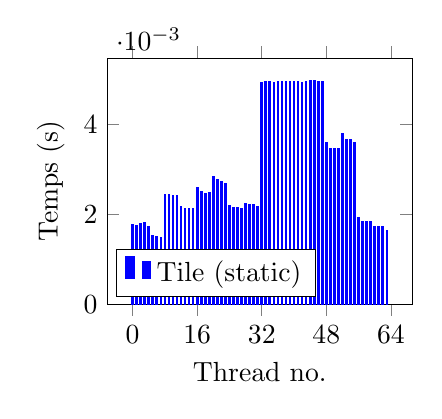
\begin{tikzpicture}
\begin{axis}[
  ybar,
  bar width=0.02cm,
  xlabel={Thread no.},
  ylabel={Temps (s)},
  ymin=0,
  legend pos=south west,
  width=0.45\textwidth,
  xtick distance=16
]

% Données pour le premier graphique (à gauche)
\addplot[color=blue, fill=blue] coordinates {
  (0,0.001768) (1,0.001749) (2,0.001797) (3,0.001820) (4,0.001723) (5,0.001518) (6,0.001508) (7,0.001492) (8,0.002447) (9,0.002438) (10,0.002415) (11,0.002412) (12,0.002181) (13,0.002134) (14,0.002132) (15,0.002121) (16,0.002595) (17,0.002512) (18,0.002463) (19,0.002481) (20,0.002849) (21,0.002782) (22,0.002726) (23,0.002688) (24,0.002196) (25,0.002153) (26,0.002149) (27,0.002128) (28,0.002237) (29,0.002208) (30,0.002205) (31,0.002172) (32,0.004938) (33,0.004952) (34,0.004951) (35,0.004932) (36,0.004957) (37,0.004956) (38,0.004958) (39,0.004951) (40,0.004945) (41,0.004945) (42,0.004939) (43,0.004944) (44,0.004967) (45,0.004975) (46,0.004953) (47,0.004945) (48,0.003589) (49,0.003467) (50,0.003454) (51,0.003460) (52,0.003787) (53,0.003659) (54,0.003653) (55,0.003591) (56,0.001933) (57,0.001843) (58,0.001843) (59,0.001828) (60,0.001734) (61,0.001733) (62,0.001731) (63,0.001631)
};
\addlegendentry{Tile (static)}

\end{axis}
\end{tikzpicture}
\hfill
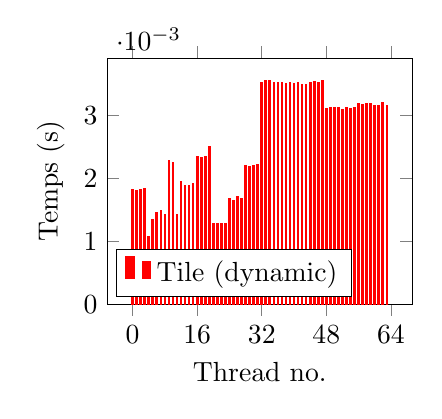
\begin{tikzpicture}
\begin{axis}[
  ybar,
  bar width=0.02cm,
  xlabel={Thread no.},
  ylabel={Temps (s)},
  ymin=0,
  legend pos=south west,
  width=0.45\textwidth,
  xtick distance=16
]

% Données pour le deuxième graphique (au milieu)
\addplot[color=red, fill=red] coordinates {
  (0,0.001829) (1,0.001812) (2,0.001827) (3,0.001834) (4,0.001075) (5,0.001339) (6,0.001461) (7,0.001489) (8,0.001431) (9,0.002278) (10,0.002259) (11,0.001431) (12,0.001946) (13,0.001890) (14,0.001879) (15,0.001911) (16,0.002345) (17,0.002334) (18,0.002350) (19,0.002506) (20,0.001287) (21,0.001288) (22,0.001287) (23,0.001287) (24,0.001678) (25,0.001655) (26,0.001714) (27,0.001676) (28,0.002199) (29,0.002193) (30,0.002200) (31,0.002217) (32,0.003526) (33,0.003554) (34,0.003557) (35,0.003525) (36,0.003530) (37,0.003529) (38,0.003514) (39,0.003531) (40,0.003511) (41,0.003530) (42,0.003498) (43,0.003499) (44,0.003523) (45,0.003540) (46,0.003524) (47,0.003550) (48,0.003112) (49,0.003122) (50,0.003126) (51,0.003130) (52,0.003102) (53,0.003125) (54,0.003104) (55,0.003123) (56,0.003197) (57,0.003180) (58,0.003189) (59,0.003191) (60,0.003156) (61,0.003166) (62,0.003205) (63,0.003154)
};
\addlegendentry{Tile (dynamic)}

\end{axis}
\end{tikzpicture}
\hfill
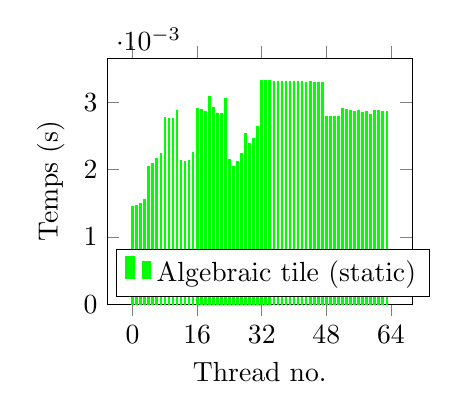
\begin{tikzpicture}
\begin{axis}[
  ybar,
  bar width=0.02cm,
  xlabel={Thread no.},
  ylabel={Temps (s)},
  ymin=0,
  legend pos=south west,
  width=0.45\textwidth,
  xtick distance=16
]

% Données pour le troisième graphique (à droite)
\addplot[color=green, fill=green] coordinates {
  (0,0.001449) (1,0.001464) (2,0.001501) (3,0.001561) (4,0.002043) (5,0.002087) (6,0.002170) (7,0.002237) (8,0.002774) (9,0.002766) (10,0.002758) (11,0.002876) (12,0.002140) (13,0.002119) (14,0.002138) (15,0.002252) (16,0.002908) (17,0.002898) (18,0.002860) (19,0.003085) (20,0.002924) (21,0.002836) (22,0.002840) (23,0.003052) (24,0.002148) (25,0.002039) (26,0.002126) (27,0.002234) (28,0.002544) (29,0.002385) (30,0.002456) (31,0.002647) (32,0.003319) (33,0.003319) (34,0.003326) (35,0.003307) (36,0.003315) (37,0.003310) (38,0.003311) (39,0.003307) (40,0.003308) (41,0.003315) (42,0.003317) (43,0.003289) (44,0.003306) (45,0.003301) (46,0.003301) (47,0.003292) (48,0.002791) (49,0.002785) (50,0.002791) (51,0.002783) (52,0.002906) (53,0.002897) (54,0.002880) (55,0.002859) (56,0.002872) (57,0.002854) (58,0.002859) (59,0.002826) (60,0.002875) (61,0.002880) (62,0.002867) (63,0.002863)
};
\addlegendentry{Algebraic tile (static)}

\end{axis}
\end{tikzpicture}

\caption{Temps d'exécution des threads pour le fichier atax.c}
\label{fig:graphes}
\end{figure}

\begin{table}[htbp]
  \centering
  \caption{Statistiques pour le fichier atax.c}
  \begin{tabular}{|c|c|c|c|}
    \hline
    Statistique & Algebraic Tile & Tile (static) & Tile (dynamic) \\ 
    \hline
    Skewness (g1)  & -0.834229 & 0.607996 & -0.23709 \\ 
    Kurtosis (g2)  & 0.00713479 & -1.21837 & -1.49105 \\ 
    Coefficient de variation $ \frac{\sigma}{\overline{x}} $ & 0.186052 & 0.417271 & 0.319963\\ 
    Percent Imbalance metric en \% & 21.7423 & 65.5376 & 38.1944\\ 
    Coefficient de Gini  & 0.100788 & 0.227702 & 0.179983\\ 
    Temps d'exécution (s) &  0.003410    &  0.005049   &  0.003644   \\ 

    \hline
  \end{tabular}
\end{table}
g1=$ \frac{\sum_{i=1}^{n} (x_i - \overline{x})^3}{n\sigma^3} $\
g2=$ \frac{\sum_{i=1}^{n} (x_i - \overline{x})^4}{n\sigma^4} $\
Coefficient de Gini = $ \frac{\sum_{i=1}^{n}\sum_{j=1}^{n} |x_i - x_j|}{2n^2\overline{x}} $\
\newpage

\begin{figure}
\centering

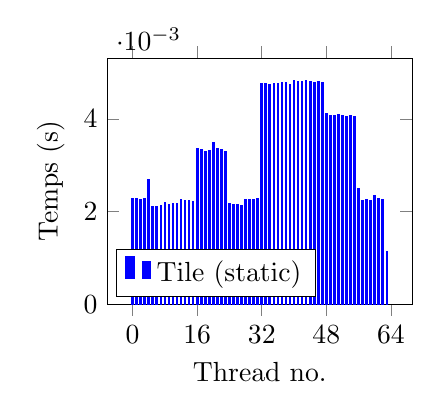
\begin{tikzpicture}
\begin{axis}[
  ybar,
  bar width=0.02cm,
  xlabel={Thread no.},
  ylabel={Temps (s)},
  ymin=0,
  legend pos=south west,
  width=0.45\textwidth,
  xtick distance=16
]

% Données pour le premier graphique (à gauche)
\addplot[color=blue, fill=blue] coordinates {
  (0,0.002275) (1,0.002272) (2,0.002265) (3,0.002282) (4,0.002697) (5,0.002101) (6,0.002114) (7,0.002138) (8,0.002184) (9,0.002160) (10,0.002162) (11,0.002165) (12,0.002262) (13,0.002239) (14,0.002227) (15,0.002213) (16,0.003363) (17,0.003338) (18,0.003297) (19,0.003306) (20,0.003482) (21,0.003359) (22,0.003334) (23,0.003300) (24,0.002174) (25,0.002141) (26,0.002144) (27,0.002132) (28,0.002262) (29,0.002261) (30,0.002263) (31,0.002277) (32,0.004752) (33,0.004764) (34,0.004740) (35,0.004754) (36,0.004772) (37,0.004786) (38,0.004775) (39,0.004747) (40,0.004827) (41,0.004812) (42,0.004814) (43,0.004828) (44,0.004799) (45,0.004793) (46,0.004803) (47,0.004793) (48,0.004107) (49,0.004081) (50,0.004079) (51,0.004084) (52,0.004066) (53,0.004044) (54,0.004062) (55,0.004056) (56,0.002493) (57,0.002239) (58,0.002252) (59,0.002239) (60,0.002336) (61,0.002278) (62,0.002249) (63,0.001126)
};
\addlegendentry{Tile (static)}

\end{axis}
\end{tikzpicture}
\hfill
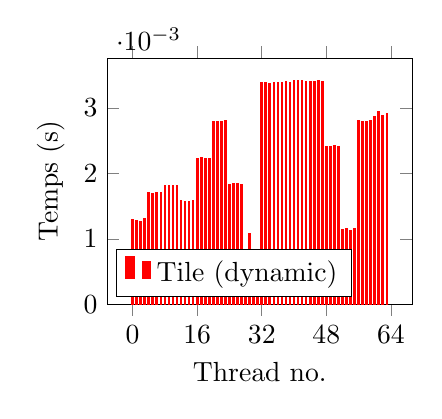
\begin{tikzpicture}
\begin{axis}[
  ybar,
  bar width=0.02cm,
  xlabel={Thread no.},
  ylabel={Temps (s)},
  ymin=0,
  legend pos=south west,
  width=0.45\textwidth,
  xtick distance=16
]

% Données pour le deuxième graphique (au milieu)
\addplot[color=red, fill=red] coordinates {
  (0,0.001289) (1,0.001277) (2,0.001269) (3,0.001310) (4,0.001705) (5,0.001692) (6,0.001706) (7,0.001711) (8,0.001816) (9,0.001821) (10,0.001809) (11,0.001809) (12,0.001581) (13,0.001570) (14,0.001568) (15,0.001585) (16,0.002231) (17,0.002243) (18,0.002234) (19,0.002231) (20,0.002795) (21,0.002795) (22,0.002796) (23,0.002813) (24,0.001837) (25,0.001850) (26,0.001849) (27,0.001836) (28,0.000727) (29,0.001082) (30,0.000731) (31,0.000724) (32,0.003393) (33,0.003389) (34,0.003378) (35,0.003394) (36,0.003388) (37,0.003391) (38,0.003405) (39,0.003387) (40,0.003418) (41,0.003421) (42,0.003420) (43,0.003412) (44,0.003409) (45,0.003409) (46,0.003413) (47,0.003410) (48,0.002414) (49,0.002411) (50,0.002430) (51,0.002411) (52,0.001146) (53,0.001151) (54,0.001125) (55,0.001149) (56,0.002806) (57,0.002795) (58,0.002795) (59,0.002807) (60,0.002874) (61,0.002940) (62,0.002883) (63,0.002910)
};
\addlegendentry{Tile (dynamic)}

\end{axis}
\end{tikzpicture}
\hfill
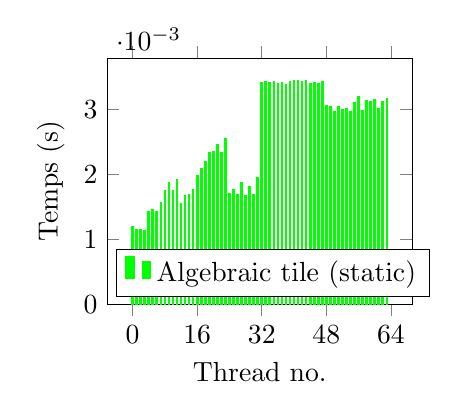
\begin{tikzpicture}
\begin{axis}[
  ybar,
  bar width=0.02cm,
  xlabel={Thread no.},
  ylabel={Temps (s)},
  ymin=0,
  legend pos=south west,
  width=0.45\textwidth,
  xtick distance=16
]

% Données pour le troisième graphique (à droite)
\addplot[color=green, fill=green] coordinates {
  (0,0.001197) (1,0.001148) (2,0.001158) (3,0.001142) (4,0.001425) (5,0.001466) (6,0.001433) (7,0.001567) (8,0.001759) (9,0.001877) (10,0.001746) (11,0.001917) (12,0.001547) (13,0.001682) (14,0.001687) (15,0.001771) (16,0.001977) (17,0.002099) (18,0.002197) (19,0.002337) (20,0.002351) (21,0.002460) (22,0.002337) (23,0.002554) (24,0.001704) (25,0.001775) (26,0.001692) (27,0.001880) (28,0.001678) (29,0.001807) (30,0.001684) (31,0.001957) (32,0.003427) (33,0.003428) (34,0.003413) (35,0.003435) (36,0.003408) (37,0.003417) (38,0.003396) (39,0.003436) (40,0.003443) (41,0.003451) (42,0.003429) (43,0.003449) (44,0.003400) (45,0.003412) (46,0.003406) (47,0.003439) (48,0.003063) (49,0.003056) (50,0.002970) (51,0.003053) (52,0.002997) (53,0.003020) (54,0.002966) (55,0.003115) (56,0.003197) (57,0.002984) (58,0.003135) (59,0.003122) (60,0.003162) (61,0.003021) (62,0.003127) (63,0.003174)
};
\addlegendentry{Algebraic tile (static)}

\end{axis}
\end{tikzpicture}

\caption{Temps d'exécution des threads pour le fichier bicg.c}
\label{fig:graphes}
\end{figure}

\begin{table}[htbp]
  \centering
  \caption{Statistiques pour le fichier bicg.c}
  \begin{tabular}{|c|c|c|c|}
    \hline
    Statistique & Algebraic Tile & Tile (static) & Tile (dynamic) \\ 
    \hline
    Skewness (g1)  & -0.224557 & 0.286089 & -0.125401 \\ 
    Kurtosis (g2)  & -1.52177 & -1.49357 & -1.26994 \\ 
    Coefficient de variation $ \frac{\sigma}{\overline{x}} $ & 0.314069 & 0.345588 & 0.369707\\ 
    Percent Imbalance metric en \% & 37.2151 & 49.6048 & 48.1594\\ 
    Coefficient de Gini  & 0.176533 & 0.189339 & 0.210629\\ 
    Temps d'exécution (s) &  0.003538    &  0.004926   &  0.003514   \\ 

    \hline
  \end{tabular}
\end{table}
g1=$ \frac{\sum_{i=1}^{n} (x_i - \overline{x})^3}{n\sigma^3} $\
g2=$ \frac{\sum_{i=1}^{n} (x_i - \overline{x})^4}{n\sigma^4} $\
Coefficient de Gini = $ \frac{\sum_{i=1}^{n}\sum_{j=1}^{n} |x_i - x_j|}{2n^2\overline{x}} $\
\newpage

\begin{figure}
\centering

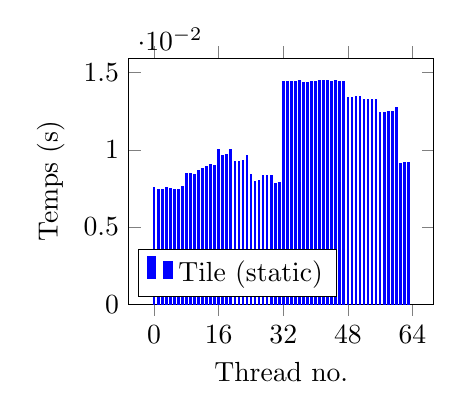
\begin{tikzpicture}
\begin{axis}[
  ybar,
  bar width=0.02cm,
  xlabel={Thread no.},
  ylabel={Temps (s)},
  ymin=0,
  legend pos=south west,
  width=0.45\textwidth,
  xtick distance=16
]

% Données pour le premier graphique (à gauche)
\addplot[color=blue, fill=blue] coordinates {
  (0,0.007559) (1,0.007442) (2,0.007453) (3,0.007583) (4,0.007498) (5,0.007449) (6,0.007461) (7,0.007655) (8,0.008450) (9,0.008489) (10,0.008416) (11,0.008689) (12,0.008791) (13,0.008905) (14,0.009040) (15,0.008996) (16,0.010013) (17,0.009648) (18,0.009705) (19,0.010020) (20,0.009273) (21,0.009265) (22,0.009284) (23,0.009637) (24,0.008408) (25,0.007955) (26,0.007999) (27,0.008330) (28,0.008307) (29,0.008324) (30,0.007831) (31,0.007905) (32,0.014410) (33,0.014417) (34,0.014430) (35,0.014430) (36,0.014487) (37,0.014383) (38,0.014396) (39,0.014409) (40,0.014453) (41,0.014468) (42,0.014476) (43,0.014484) (44,0.014447) (45,0.014499) (46,0.014450) (47,0.014458) (48,0.013409) (49,0.013422) (50,0.013432) (51,0.013457) (52,0.013244) (53,0.013281) (54,0.013251) (55,0.013278) (56,0.012429) (57,0.012429) (58,0.012455) (59,0.012478) (60,0.012728) (61,0.009130) (62,0.009151) (63,0.009167)
};
\addlegendentry{Tile (static)}

\end{axis}
\end{tikzpicture}
\hfill
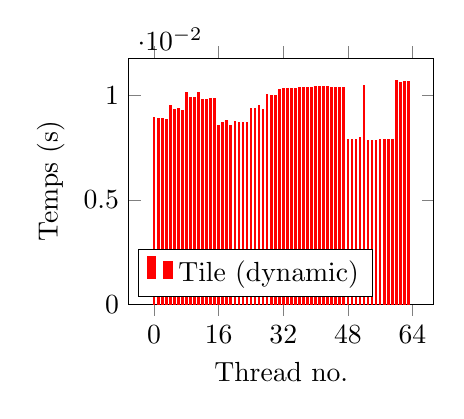
\begin{tikzpicture}
\begin{axis}[
  ybar,
  bar width=0.02cm,
  xlabel={Thread no.},
  ylabel={Temps (s)},
  ymin=0,
  legend pos=south west,
  width=0.45\textwidth,
  xtick distance=16
]

% Données pour le deuxième graphique (au milieu)
\addplot[color=red, fill=red] coordinates {
  (0,0.008933) (1,0.008889) (2,0.008915) (3,0.008841) (4,0.009542) (5,0.009347) (6,0.009397) (7,0.009311) (8,0.010160) (9,0.009901) (10,0.009899) (11,0.010148) (12,0.009812) (13,0.009817) (14,0.009872) (15,0.009864) (16,0.008590) (17,0.008734) (18,0.008800) (19,0.008560) (20,0.008769) (21,0.008704) (22,0.008699) (23,0.008734) (24,0.009362) (25,0.009369) (26,0.009511) (27,0.009348) (28,0.010045) (29,0.010017) (30,0.010002) (31,0.010281) (32,0.010321) (33,0.010324) (34,0.010326) (35,0.010320) (36,0.010386) (37,0.010386) (38,0.010387) (39,0.010387) (40,0.010418) (41,0.010418) (42,0.010419) (43,0.010419) (44,0.010397) (45,0.010397) (46,0.010399) (47,0.010397) (48,0.007915) (49,0.007920) (50,0.007919) (51,0.007985) (52,0.010464) (53,0.007826) (54,0.007832) (55,0.007830) (56,0.007901) (57,0.007899) (58,0.007910) (59,0.007901) (60,0.010729) (61,0.010649) (62,0.010671) (63,0.010671)
};
\addlegendentry{Tile (dynamic)}

\end{axis}
\end{tikzpicture}
\hfill
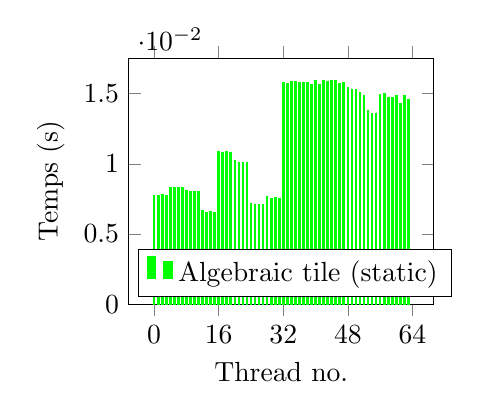
\begin{tikzpicture}
\begin{axis}[
  ybar,
  bar width=0.02cm,
  xlabel={Thread no.},
  ylabel={Temps (s)},
  ymin=0,
  legend pos=south west,
  width=0.45\textwidth,
  xtick distance=16
]

% Données pour le troisième graphique (à droite)
\addplot[color=green, fill=green] coordinates {
  (0,0.007750) (1,0.007748) (2,0.007811) (3,0.007765) (4,0.008332) (5,0.008273) (6,0.008322) (7,0.008281) (8,0.008111) (9,0.008002) (10,0.008038) (11,0.008016) (12,0.006660) (13,0.006545) (14,0.006603) (15,0.006537) (16,0.010898) (17,0.010766) (18,0.010882) (19,0.010769) (20,0.010214) (21,0.010096) (22,0.010100) (23,0.010074) (24,0.007177) (25,0.007069) (26,0.007113) (27,0.007066) (28,0.007676) (29,0.007527) (30,0.007572) (31,0.007488) (32,0.015817) (33,0.015745) (34,0.015857) (35,0.015836) (36,0.015789) (37,0.015800) (38,0.015775) (39,0.015632) (40,0.015933) (41,0.015628) (42,0.015901) (43,0.015834) (44,0.015898) (45,0.015921) (46,0.015705) (47,0.015821) (48,0.015419) (49,0.015284) (50,0.015293) (51,0.015100) (52,0.014827) (53,0.013773) (54,0.013572) (55,0.013575) (56,0.014930) (57,0.014977) (58,0.014733) (59,0.014728) (60,0.014828) (61,0.014312) (62,0.014883) (63,0.014596)
};
\addlegendentry{Algebraic tile (static)}

\end{axis}
\end{tikzpicture}

\caption{Temps d'exécution des threads pour le fichier mvt.c}
\label{fig:graphes}
\end{figure}

\begin{table}[htbp]
  \centering
  \caption{Statistiques pour le fichier mvt.c}
  \begin{tabular}{|c|c|c|c|}
    \hline
    Statistique & Algebraic Tile & Tile (static) & Tile (dynamic) \\ 
    \hline
    Skewness (g1)  & -0.133745 & 0.153532 & -0.481354 \\ 
    Kurtosis (g2)  & -1.74893 & -1.7022 & -1.15839 \\ 
    Coefficient de variation $ \frac{\sigma}{\overline{x}} $ & 0.309467 & 0.249715 & 0.099745\\ 
    Percent Imbalance metric en \% & 35.4191 & 32.635 & 13.2542\\ 
    Coefficient de Gini  & 0.171333 & 0.139091 & 0.0559441\\ 
    Temps d'exécution (s) &  0.016057    &  0.014598   &  0.010810   \\ 

    \hline
  \end{tabular}
\end{table}
g1=$ \frac{\sum_{i=1}^{n} (x_i - \overline{x})^3}{n\sigma^3} $\
g2=$ \frac{\sum_{i=1}^{n} (x_i - \overline{x})^4}{n\sigma^4} $\
Coefficient de Gini = $ \frac{\sum_{i=1}^{n}\sum_{j=1}^{n} |x_i - x_j|}{2n^2\overline{x}} $\
\newpage

\begin{figure}
\centering

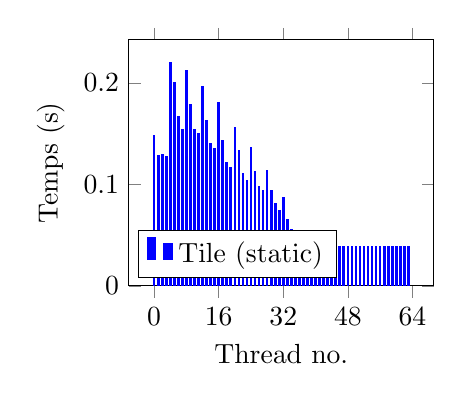
\begin{tikzpicture}
\begin{axis}[
  ybar,
  bar width=0.02cm,
  xlabel={Thread no.},
  ylabel={Temps (s)},
  ymin=0,
  legend pos=south west,
  width=0.45\textwidth,
  xtick distance=16
]

% Données pour le premier graphique (à gauche)
\addplot[color=blue, fill=blue] coordinates {
  (0,0.148252) (1,0.128778) (2,0.129615) (3,0.127699) (4,0.220657) (5,0.200751) (6,0.166860) (7,0.153821) (8,0.211909) (9,0.178686) (10,0.154392) (11,0.149711) (12,0.196499) (13,0.162747) (14,0.140346) (15,0.135145) (16,0.180303) (17,0.143632) (18,0.121623) (19,0.117050) (20,0.156034) (21,0.133528) (22,0.111208) (23,0.103583) (24,0.136634) (25,0.112675) (26,0.097470) (27,0.093582) (28,0.113714) (29,0.094196) (30,0.081490) (31,0.074218) (32,0.086575) (33,0.065640) (34,0.055549) (35,0.051495) (36,0.053374) (37,0.043151) (38,0.038299) (39,0.038256) (40,0.038850) (41,0.038815) (42,0.038881) (43,0.038882) (44,0.038882) (45,0.038812) (46,0.038912) (47,0.038873) (48,0.038762) (49,0.038769) (50,0.038827) (51,0.038823) (52,0.038797) (53,0.038781) (54,0.038823) (55,0.038796) (56,0.038947) (57,0.038974) (58,0.038932) (59,0.038933) (60,0.038925) (61,0.038930) (62,0.038985) (63,0.038929)
};
\addlegendentry{Tile (static)}

\end{axis}
\end{tikzpicture}
\hfill
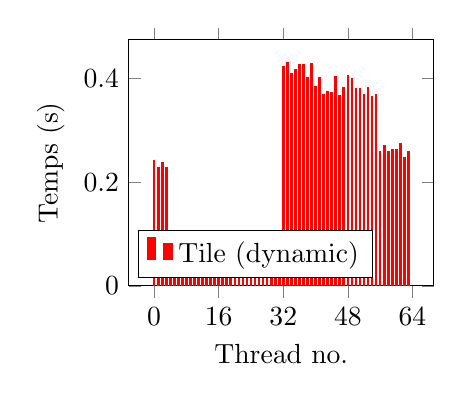
\begin{tikzpicture}
\begin{axis}[
  ybar,
  bar width=0.02cm,
  xlabel={Thread no.},
  ylabel={Temps (s)},
  ymin=0,
  legend pos=south west,
  width=0.45\textwidth,
  xtick distance=16
]

% Données pour le deuxième graphique (au milieu)
\addplot[color=red, fill=red] coordinates {
  (0,0.242409) (1,0.228284) (2,0.238842) (3,0.228829) (4,0.064033) (5,0.066269) (6,0.060129) (7,0.066274) (8,0.041526) (9,0.041867) (10,0.042079) (11,0.042243) (12,0.041599) (13,0.041564) (14,0.041604) (15,0.041580) (16,0.081268) (17,0.089029) (18,0.072700) (19,0.072314) (20,0.076032) (21,0.079314) (22,0.074039) (23,0.070894) (24,0.046147) (25,0.045386) (26,0.044717) (27,0.044308) (28,0.046397) (29,0.047124) (30,0.045553) (31,0.047015) (32,0.424301) (33,0.432112) (34,0.409970) (35,0.418067) (36,0.427305) (37,0.427695) (38,0.402580) (39,0.430003) (40,0.384386) (41,0.401748) (42,0.370322) (43,0.375591) (44,0.373664) (45,0.404570) (46,0.366749) (47,0.383557) (48,0.405398) (49,0.399511) (50,0.381502) (51,0.381619) (52,0.369075) (53,0.382277) (54,0.365149) (55,0.370354) (56,0.258585) (57,0.271323) (58,0.259338) (59,0.262929) (60,0.263114) (61,0.274583) (62,0.248464) (63,0.258497)
};
\addlegendentry{Tile (dynamic)}

\end{axis}
\end{tikzpicture}
\hfill
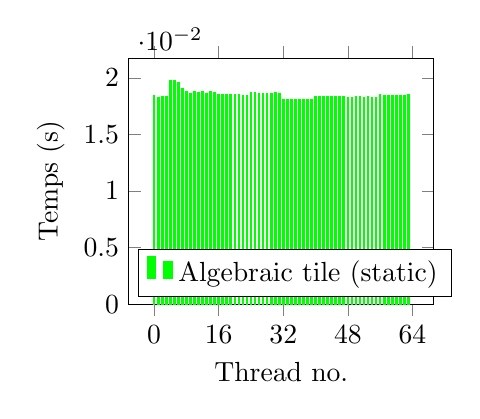
\begin{tikzpicture}
\begin{axis}[
  ybar,
  bar width=0.02cm,
  xlabel={Thread no.},
  ylabel={Temps (s)},
  ymin=0,
  legend pos=south west,
  width=0.45\textwidth,
  xtick distance=16
]

% Données pour le troisième graphique (à droite)
\addplot[color=green, fill=green] coordinates {
  (0,0.018409) (1,0.018282) (2,0.018345) (3,0.018323) (4,0.019756) (5,0.019779) (6,0.019612) (7,0.019038) (8,0.018794) (9,0.018661) (10,0.018821) (11,0.018734) (12,0.018781) (13,0.018648) (14,0.018774) (15,0.018735) (16,0.018500) (17,0.018518) (18,0.018535) (19,0.018544) (20,0.018552) (21,0.018502) (22,0.018458) (23,0.018446) (24,0.018718) (25,0.018684) (26,0.018651) (27,0.018645) (28,0.018652) (29,0.018656) (30,0.018705) (31,0.018662) (32,0.018073) (33,0.018094) (34,0.018081) (35,0.018067) (36,0.018063) (37,0.018067) (38,0.018093) (39,0.018063) (40,0.018368) (41,0.018323) (42,0.018383) (43,0.018364) (44,0.018376) (45,0.018327) (46,0.018383) (47,0.018371) (48,0.018284) (49,0.018307) (50,0.018333) (51,0.018358) (52,0.018312) (53,0.018321) (54,0.018288) (55,0.018294) (56,0.018503) (57,0.018487) (58,0.018449) (59,0.018411) (60,0.018430) (61,0.018462) (62,0.018483) (63,0.018516)
};
\addlegendentry{Algebraic tile (static)}

\end{axis}
\end{tikzpicture}

\caption{Temps d'exécution des threads pour le fichier gramschmidt.c}
\label{fig:graphes}
\end{figure}

\begin{table}[htbp]
  \centering
  \caption{Statistiques pour le fichier gramschmidt.c}
  \begin{tabular}{|c|c|c|c|}
    \hline
    Statistique & Algebraic Tile & Tile (static) & Tile (dynamic) \\ 
    \hline
    Skewness (g1)  & 1.88286 & 0.58724 & 0.0379406 \\ 
    Kurtosis (g2)  & 4.84445 & -0.937669 & -1.72775 \\ 
    Coefficient de variation $ \frac{\sigma}{\overline{x}} $ & 0.0184978 & 0.60775 & 0.700429\\ 
    Percent Imbalance metric en \% & 6.8546 & 141.734 & 96.1961\\ 
    Coefficient de Gini  & 0.00908493 & 0.332126 & 0.387914\\ 
    Temps d'exécution (s) &  0.025506    &  0.255638   &  0.672374   \\ 

    \hline
  \end{tabular}
\end{table}
g1=$ \frac{\sum_{i=1}^{n} (x_i - \overline{x})^3}{n\sigma^3} $\
g2=$ \frac{\sum_{i=1}^{n} (x_i - \overline{x})^4}{n\sigma^4} $\
Coefficient de Gini = $ \frac{\sum_{i=1}^{n}\sum_{j=1}^{n} |x_i - x_j|}{2n^2\overline{x}} $\
\newpage

\begin{figure}
\centering

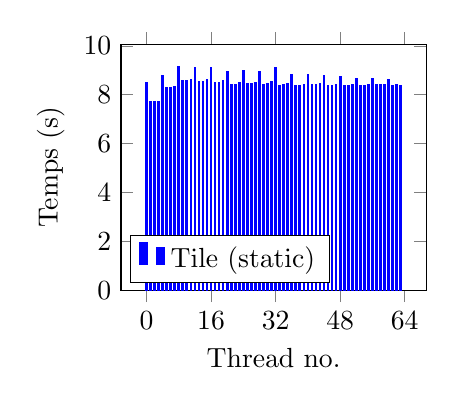
\begin{tikzpicture}
\begin{axis}[
  ybar,
  bar width=0.02cm,
  xlabel={Thread no.},
  ylabel={Temps (s)},
  ymin=0,
  legend pos=south west,
  width=0.45\textwidth,
  xtick distance=16
]

% Données pour le premier graphique (à gauche)
\addplot[color=blue, fill=blue] coordinates {
  (0,8.482317) (1,7.730170) (2,7.722670) (3,7.737962) (4,8.777212) (5,8.303672) (6,8.308033) (7,8.321441) (8,9.149074) (9,8.567041) (10,8.571775) (11,8.632985) (12,9.098212) (13,8.536508) (14,8.544569) (15,8.611480) (16,9.117206) (17,8.489650) (18,8.492718) (19,8.558366) (20,8.963380) (21,8.432489) (22,8.433589) (23,8.494456) (24,8.978987) (25,8.463076) (26,8.451214) (27,8.515799) (28,8.944131) (29,8.431922) (30,8.450613) (31,8.544253) (32,9.093508) (33,8.386975) (34,8.397215) (35,8.463645) (36,8.827246) (37,8.373002) (38,8.380398) (39,8.432193) (40,8.840198) (41,8.412735) (42,8.409549) (43,8.466501) (44,8.772989) (45,8.385594) (46,8.381016) (47,8.434263) (48,8.762061) (49,8.385673) (50,8.387621) (51,8.418859) (52,8.655843) (53,8.374267) (54,8.393699) (55,8.401431) (56,8.660495) (57,8.412290) (58,8.417729) (59,8.434729) (60,8.601711) (61,8.394107) (62,8.407856) (63,8.392190)
};
\addlegendentry{Tile (static)}

\end{axis}
\end{tikzpicture}
\hfill
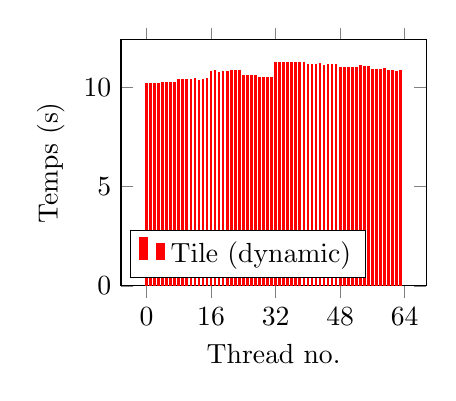
\begin{tikzpicture}
\begin{axis}[
  ybar,
  bar width=0.02cm,
  xlabel={Thread no.},
  ylabel={Temps (s)},
  ymin=0,
  legend pos=south west,
  width=0.45\textwidth,
  xtick distance=16
]

% Données pour le deuxième graphique (au milieu)
\addplot[color=red, fill=red] coordinates {
  (0,10.214788) (1,10.197535) (2,10.194933) (3,10.199989) (4,10.218227) (5,10.223842) (6,10.216741) (7,10.225611) (8,10.366577) (9,10.404087) (10,10.388027) (11,10.375935) (12,10.419370) (13,10.359944) (14,10.391113) (15,10.421537) (16,10.813647) (17,10.835562) (18,10.766120) (19,10.807119) (20,10.819533) (21,10.852203) (22,10.827648) (23,10.845226) (24,10.575628) (25,10.605084) (26,10.572913) (27,10.585534) (28,10.472600) (29,10.497409) (30,10.479083) (31,10.491299) (32,11.253234) (33,11.269749) (34,11.249365) (35,11.258380) (36,11.256848) (37,11.245216) (38,11.223938) (39,11.250552) (40,11.126715) (41,11.142370) (42,11.144799) (43,11.176547) (44,11.098074) (45,11.124484) (46,11.127838) (47,11.161391) (48,10.975917) (49,10.985437) (50,10.972807) (51,10.975247) (52,11.018257) (53,11.074055) (54,11.024233) (55,11.027171) (56,10.895677) (57,10.897120) (58,10.890884) (59,10.930790) (60,10.839250) (61,10.822573) (62,10.810038) (63,10.825672)
};
\addlegendentry{Tile (dynamic)}

\end{axis}
\end{tikzpicture}
\hfill
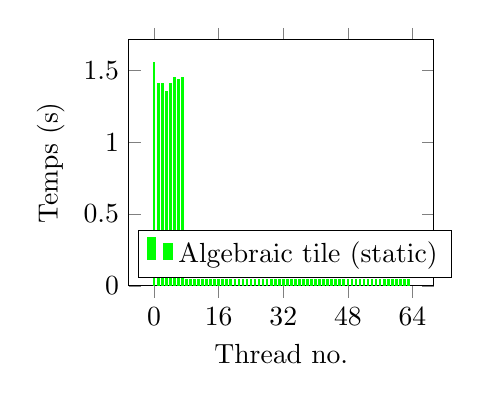
\begin{tikzpicture}
\begin{axis}[
  ybar,
  bar width=0.02cm,
  xlabel={Thread no.},
  ylabel={Temps (s)},
  ymin=0,
  legend pos=south west,
  width=0.45\textwidth,
  xtick distance=16
]

% Données pour le troisième graphique (à droite)
\addplot[color=green, fill=green] coordinates {
  (0,1.556495) (1,1.410295) (2,1.409131) (3,1.354825) (4,1.406772) (5,1.450604) (6,1.433764) (7,1.449527) (8,0.046363) (9,0.046324) (10,0.046387) (11,0.046324) (12,0.046346) (13,0.046277) (14,0.046326) (15,0.046337) (16,0.045813) (17,0.045764) (18,0.045838) (19,0.045826) (20,0.045941) (21,0.045928) (22,0.045971) (23,0.045886) (24,0.045913) (25,0.045867) (26,0.045906) (27,0.045881) (28,0.046189) (29,0.046174) (30,0.046225) (31,0.046243) (32,0.044526) (33,0.044514) (34,0.044550) (35,0.044537) (36,0.045055) (37,0.045063) (38,0.045104) (39,0.045113) (40,0.045265) (41,0.045290) (42,0.045271) (43,0.045270) (44,0.045368) (45,0.045351) (46,0.045427) (47,0.045429) (48,0.045588) (49,0.045584) (50,0.045629) (51,0.045613) (52,0.045120) (53,0.045132) (54,0.045138) (55,0.045145) (56,0.045782) (57,0.045896) (58,0.045810) (59,0.045780) (60,0.045696) (61,0.045699) (62,0.045747) (63,0.045733)
};
\addlegendentry{Algebraic tile (static)}

\end{axis}
\end{tikzpicture}

\caption{Temps d'exécution des threads pour le fichier floyd-warshall.c}
\label{fig:graphes}
\end{figure}

\begin{table}[htbp]
  \centering
  \caption{Statistiques pour le fichier floyd-warshall.c}
  \begin{tabular}{|c|c|c|c|}
    \hline
    Statistique & Algebraic Tile & Tile (static) & Tile (dynamic) \\ 
    \hline
    Skewness (g1)  & 2.27594 & -0.167246 & -0.26637 \\ 
    Kurtosis (g2)  & 3.19719 & 2.00292 & -1.22614 \\ 
    Coefficient de variation $ \frac{\sigma}{\overline{x}} $ & 2.09658 & 0.0322639 & 0.0320072\\ 
    Percent Imbalance metric en \% & 610.135 & 7.4752 & 4.57029\\ 
    Coefficient de Gini  & 0.695727 & 0.0161424 & 0.0182648\\ 
    Temps d'exécution (s) &  1.568830    &  11.195399   &  14.316092   \\ 

    \hline
  \end{tabular}
\end{table}
g1=$ \frac{\sum_{i=1}^{n} (x_i - \overline{x})^3}{n\sigma^3} $\
g2=$ \frac{\sum_{i=1}^{n} (x_i - \overline{x})^4}{n\sigma^4} $\
Coefficient de Gini = $ \frac{\sum_{i=1}^{n}\sum_{j=1}^{n} |x_i - x_j|}{2n^2\overline{x}} $\
\newpage

\begin{figure}
\centering

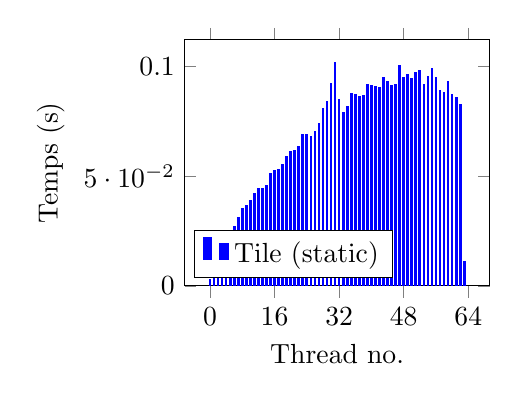
\begin{tikzpicture}
\begin{axis}[
  ybar,
  bar width=0.02cm,
  xlabel={Thread no.},
  ylabel={Temps (s)},
  ymin=0,
  legend pos=south west,
  width=0.45\textwidth,
  xtick distance=16
]

% Données pour le premier graphique (à gauche)
\addplot[color=blue, fill=blue] coordinates {
  (0,0.002634) (1,0.006714) (2,0.011025) (3,0.015839) (4,0.020638) (5,0.023267) (6,0.026894) (7,0.031061) (8,0.035323) (9,0.036575) (10,0.039078) (11,0.042335) (12,0.044553) (13,0.044600) (14,0.045823) (15,0.051300) (16,0.052435) (17,0.052866) (18,0.055519) (19,0.059193) (20,0.061497) (21,0.061749) (22,0.063355) (23,0.069031) (24,0.069061) (25,0.068344) (26,0.070500) (27,0.074185) (28,0.080859) (29,0.084300) (30,0.092452) (31,0.102104) (32,0.084860) (33,0.079304) (34,0.081778) (35,0.087788) (36,0.087361) (37,0.086433) (38,0.086820) (39,0.091874) (40,0.091306) (41,0.091088) (42,0.090652) (43,0.095196) (44,0.093381) (45,0.091602) (46,0.091927) (47,0.100499) (48,0.095273) (49,0.096635) (50,0.094776) (51,0.097206) (52,0.098345) (53,0.091935) (54,0.095475) (55,0.099155) (56,0.094900) (57,0.089059) (58,0.088133) (59,0.093247) (60,0.087383) (61,0.085793) (62,0.082942) (63,0.011268)
};
\addlegendentry{Tile (static)}

\end{axis}
\end{tikzpicture}
\hfill
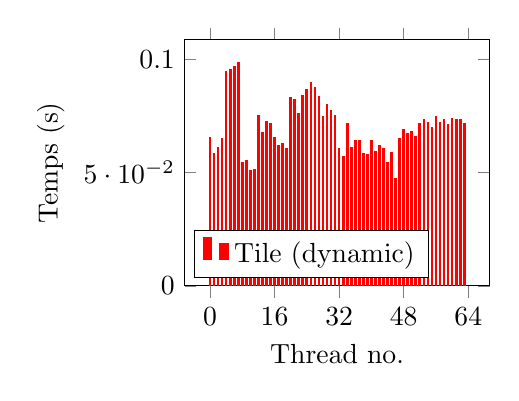
\begin{tikzpicture}
\begin{axis}[
  ybar,
  bar width=0.02cm,
  xlabel={Thread no.},
  ylabel={Temps (s)},
  ymin=0,
  legend pos=south west,
  width=0.45\textwidth,
  xtick distance=16
]

% Données pour le deuxième graphique (au milieu)
\addplot[color=red, fill=red] coordinates {
  (0,0.065311) (1,0.058151) (2,0.061041) (3,0.064846) (4,0.094446) (5,0.095358) (6,0.096586) (7,0.098662) (8,0.054224) (9,0.055382) (10,0.050873) (11,0.051446) (12,0.075077) (13,0.067380) (14,0.072397) (15,0.071744) (16,0.065338) (17,0.061647) (18,0.062950) (19,0.060327) (20,0.083121) (21,0.082170) (22,0.075948) (23,0.083816) (24,0.086404) (25,0.089853) (26,0.087551) (27,0.083364) (28,0.074748) (29,0.079849) (30,0.077095) (31,0.075201) (32,0.060595) (33,0.057143) (34,0.071547) (35,0.060823) (36,0.064007) (37,0.064081) (38,0.058352) (39,0.057880) (40,0.064063) (41,0.059417) (42,0.061661) (43,0.060616) (44,0.054583) (45,0.058618) (46,0.047257) (47,0.065090) (48,0.068713) (49,0.067352) (50,0.067844) (51,0.065643) (52,0.071610) (53,0.073298) (54,0.072175) (55,0.069825) (56,0.074746) (57,0.072178) (58,0.073200) (59,0.070933) (60,0.073867) (61,0.073429) (62,0.073255) (63,0.071521)
};
\addlegendentry{Tile (dynamic)}

\end{axis}
\end{tikzpicture}
\hfill
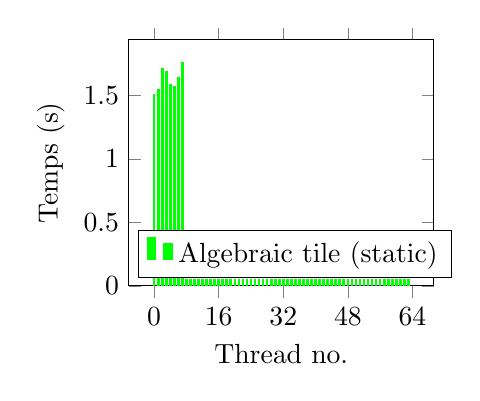
\begin{tikzpicture}
\begin{axis}[
  ybar,
  bar width=0.02cm,
  xlabel={Thread no.},
  ylabel={Temps (s)},
  ymin=0,
  legend pos=south west,
  width=0.45\textwidth,
  xtick distance=16
]

% Données pour le troisième graphique (à droite)
\addplot[color=green, fill=green] coordinates {
  (0,1.503311) (1,1.542404) (2,1.713074) (3,1.685834) (4,1.585943) (5,1.571438) (6,1.641397) (7,1.761728) (8,0.048129) (9,0.048078) (10,0.048122) (11,0.048090) (12,0.048137) (13,0.048064) (14,0.048119) (15,0.048075) (16,0.047291) (17,0.047186) (18,0.047446) (19,0.047388) (20,0.047415) (21,0.047173) (22,0.047512) (23,0.047298) (24,0.047930) (25,0.047899) (26,0.047940) (27,0.047943) (28,0.047844) (29,0.047808) (30,0.047935) (31,0.047908) (32,0.045831) (33,0.045807) (34,0.045835) (35,0.045823) (36,0.045830) (37,0.045816) (38,0.045855) (39,0.045835) (40,0.046383) (41,0.046356) (42,0.046408) (43,0.046383) (44,0.046358) (45,0.046338) (46,0.046441) (47,0.046365) (48,0.046594) (49,0.046502) (50,0.046790) (51,0.046687) (52,0.046657) (53,0.046544) (54,0.046719) (55,0.046603) (56,0.047019) (57,0.046724) (58,0.047142) (59,0.047051) (60,0.046936) (61,0.046627) (62,0.047255) (63,0.047042)
};
\addlegendentry{Algebraic tile (static)}

\end{axis}
\end{tikzpicture}

\caption{Temps d'exécution des threads pour le fichier nussinov.c}
\label{fig:graphes}
\end{figure}

\begin{table}[htbp]
  \centering
  \caption{Statistiques pour le fichier nussinov.c}
  \begin{tabular}{|c|c|c|c|}
    \hline
    Statistique & Algebraic Tile & Tile (static) & Tile (dynamic) \\ 
    \hline
    Skewness (g1)  & 2.28246 & -0.838894 & 0.566604 \\ 
    Kurtosis (g2)  & 3.23934 & -0.531387 & -0.0154646 \\ 
    Coefficient de variation $ \frac{\sigma}{\overline{x}} $ & 2.14006 & 0.404569 & 0.164252\\ 
    Percent Imbalance metric en \% & 620.985 & 47.5589 & 41.336\\ 
    Coefficient de Gini  & 0.711043 & 0.220765 & 0.0914783\\ 
    Temps d'exécution (s) &  1.799648    &  0.183833   &  0.185675   \\ 

    \hline
  \end{tabular}
\end{table}
g1=$ \frac{\sum_{i=1}^{n} (x_i - \overline{x})^3}{n\sigma^3} $\
g2=$ \frac{\sum_{i=1}^{n} (x_i - \overline{x})^4}{n\sigma^4} $\
Coefficient de Gini = $ \frac{\sum_{i=1}^{n}\sum_{j=1}^{n} |x_i - x_j|}{2n^2\overline{x}} $\
\newpage

\begin{figure}
\centering

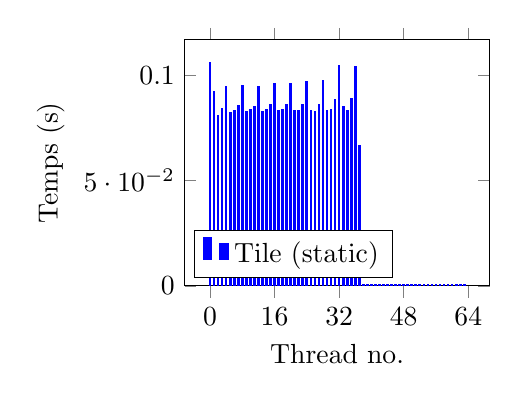
\begin{tikzpicture}
\begin{axis}[
  ybar,
  bar width=0.02cm,
  xlabel={Thread no.},
  ylabel={Temps (s)},
  ymin=0,
  legend pos=south west,
  width=0.45\textwidth,
  xtick distance=16
]

% Données pour le premier graphique (à gauche)
\addplot[color=blue, fill=blue] coordinates {
  (0,0.106154) (1,0.092129) (2,0.080739) (3,0.084230) (4,0.094619) (5,0.082335) (6,0.083336) (7,0.085673) (8,0.094821) (9,0.082766) (10,0.083479) (11,0.085146) (12,0.094599) (13,0.082462) (14,0.083702) (15,0.086060) (16,0.095850) (17,0.083055) (18,0.083604) (19,0.085953) (20,0.095841) (21,0.082971) (22,0.083030) (23,0.086128) (24,0.096804) (25,0.083045) (26,0.082905) (27,0.086182) (28,0.097456) (29,0.083332) (30,0.083730) (31,0.088264) (32,0.104631) (33,0.085131) (34,0.083176) (35,0.088840) (36,0.104236) (37,0.066660) (38,0.000561) (39,0.000562) (40,0.000575) (41,0.000574) (42,0.000574) (43,0.000574) (44,0.000571) (45,0.000571) (46,0.000570) (47,0.000570) (48,0.000573) (49,0.000574) (50,0.000574) (51,0.000573) (52,0.000574) (53,0.000578) (54,0.000576) (55,0.000576) (56,0.000572) (57,0.000574) (58,0.000571) (59,0.000575) (60,0.000577) (61,0.000577) (62,0.000577) (63,0.000574)
};
\addlegendentry{Tile (static)}

\end{axis}
\end{tikzpicture}
\hfill
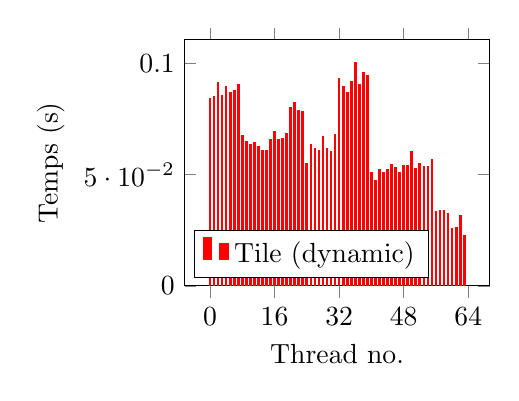
\begin{tikzpicture}
\begin{axis}[
  ybar,
  bar width=0.02cm,
  xlabel={Thread no.},
  ylabel={Temps (s)},
  ymin=0,
  legend pos=south west,
  width=0.45\textwidth,
  xtick distance=16
]

% Données pour le deuxième graphique (au milieu)
\addplot[color=red, fill=red] coordinates {
  (0,0.084177) (1,0.085272) (2,0.091700) (3,0.085831) (4,0.089810) (5,0.086828) (6,0.087995) (7,0.090489) (8,0.067624) (9,0.065012) (10,0.063811) (11,0.064685) (12,0.062837) (13,0.060886) (14,0.060835) (15,0.065816) (16,0.069443) (17,0.065678) (18,0.066223) (19,0.068529) (20,0.080076) (21,0.082469) (22,0.079129) (23,0.078581) (24,0.054834) (25,0.063495) (26,0.061683) (27,0.060805) (28,0.067162) (29,0.061622) (30,0.060357) (31,0.068143) (32,0.093122) (33,0.089727) (34,0.087251) (35,0.091875) (36,0.100733) (37,0.090725) (38,0.096108) (39,0.094711) (40,0.051073) (41,0.047354) (42,0.052362) (43,0.050828) (44,0.052552) (45,0.054419) (46,0.053090) (47,0.050861) (48,0.054303) (49,0.054111) (50,0.060277) (51,0.052813) (52,0.055077) (53,0.053917) (54,0.053619) (55,0.056780) (56,0.033652) (57,0.033699) (58,0.034107) (59,0.032737) (60,0.025592) (61,0.026088) (62,0.031666) (63,0.022802)
};
\addlegendentry{Tile (dynamic)}

\end{axis}
\end{tikzpicture}
\hfill
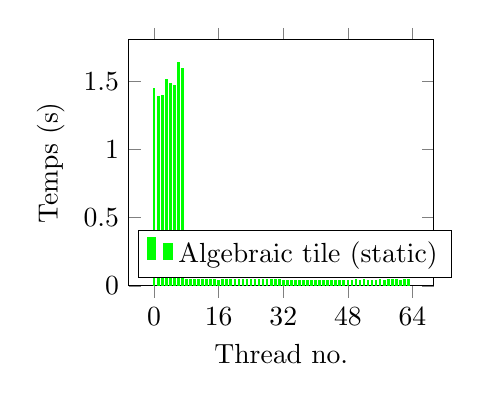
\begin{tikzpicture}
\begin{axis}[
  ybar,
  bar width=0.02cm,
  xlabel={Thread no.},
  ylabel={Temps (s)},
  ymin=0,
  legend pos=south west,
  width=0.45\textwidth,
  xtick distance=16
]

% Données pour le troisième graphique (à droite)
\addplot[color=green, fill=green] coordinates {
  (0,1.447939) (1,1.389448) (2,1.400140) (3,1.513796) (4,1.488899) (5,1.472979) (6,1.642859) (7,1.597565) (8,0.043362) (9,0.043266) (10,0.043326) (11,0.043288) (12,0.043410) (13,0.043344) (14,0.043442) (15,0.043383) (16,0.041899) (17,0.042395) (18,0.042789) (19,0.042687) (20,0.042857) (21,0.042708) (22,0.042978) (23,0.042857) (24,0.043185) (25,0.043112) (26,0.043196) (27,0.043107) (28,0.043100) (29,0.043072) (30,0.043175) (31,0.043171) (32,0.041389) (33,0.041364) (34,0.041402) (35,0.041387) (36,0.041377) (37,0.041367) (38,0.041399) (39,0.041368) (40,0.041904) (41,0.041907) (42,0.041975) (43,0.041946) (44,0.041931) (45,0.041908) (46,0.041929) (47,0.041952) (48,0.042079) (49,0.042080) (50,0.042310) (51,0.042139) (52,0.042182) (53,0.042006) (54,0.042114) (55,0.042055) (56,0.042486) (57,0.042160) (58,0.042303) (59,0.042391) (60,0.042249) (61,0.042106) (62,0.042511) (63,0.042326)
};
\addlegendentry{Algebraic tile (static)}

\end{axis}
\end{tikzpicture}

\caption{Temps d'exécution des threads pour le fichier fdtd-2d.c}
\label{fig:graphes}
\end{figure}

\begin{table}[htbp]
  \centering
  \caption{Statistiques pour le fichier fdtd-2d.c}
  \begin{tabular}{|c|c|c|c|}
    \hline
    Statistique & Algebraic Tile & Tile (static) & Tile (dynamic) \\ 
    \hline
    Skewness (g1)  & 2.28509 & -0.323751 & -0.142614 \\ 
    Kurtosis (g2)  & 3.25756 & -1.81397 & -0.619018 \\ 
    Coefficient de variation $ \frac{\sigma}{\overline{x}} $ & 2.14858 & 0.825841 & 0.299323\\ 
    Percent Imbalance metric en \% & 633.789 & 102.925 & 55.7276\\ 
    Coefficient de Gini  & 0.71376 & 0.428317 & 0.168548\\ 
    Temps d'exécution (s) &  1.669871 &  0.109399   &  0.127525   \\ 

    \hline
  \end{tabular}
\end{table}
g1=$ \frac{\sum_{i=1}^{n} (x_i - \overline{x})^3}{n\sigma^3} $\
g2=$ \frac{\sum_{i=1}^{n} (x_i - \overline{x})^4}{n\sigma^4} $\
Coefficient de Gini = $ \frac{\sum_{i=1}^{n}\sum_{j=1}^{n} |x_i - x_j|}{2n^2\overline{x}} $\
\newpage

  \end{document}
